\documentclass[12pt]{article}
\usepackage{setspace, graphicx, fullpage, amssymb, amsmath, epsfig, natbib, array, multirow, hyperref}
\usepackage{amsfonts, bm} 
\usepackage{dcolumn}
\usepackage{subfigure, float} 
\usepackage[margin=1in]{geometry} 
\usepackage{verbatim}
\usepackage{url}
\usepackage{enumerate}
\usepackage{morefloats}
\newcolumntype{d}[1]{D{.}{.}{#1}} 

\begin{document}
	
\begin{center}
	\Large 08 March 2017
\end{center}

\section{Overview}

At our previous meeting we decided to do the following:

\begin{itemize}
	\item Conduct additional analyses using fixed effects and separating out aggregate results by party and majority status
	
	\item Check variables, especially the vote share and presidential vote share
	
	\item Include past tables and figures in the weekly update to allow us to review them together more easily
\end{itemize}


I have done these things and include the results below. It should be noted that what previously appeared to be an interesting trend amongst Republicans in the House Majority in the DV/IV plots resulted from the fact that the plots of majority and minority party points were plotted together and overlapped in many cases. I apologize for not previously working to account for this and in future instances which I do such dense plots I will reduce the opacity of points so the resulting plots are not similarly misleading. The Senate fixed effects models put the sign on presidential vote share in the same direction across the board. 

I further demonstrate the variable's integrity by showing plots of it against Democratic presidential vote share (which we also have in our data). I do this for all observations and for observations broken down by party. I then show a summary table of the two party vote share variable for all Senators and decomposed by party. Note: the particularly low Democratic presidential vote shares come from the electoral routing of George McGovern in Southern states, results which I verified with outside sources. Since it is above 0.50 for all Senators (as would be expected), I remain confident that it is correctly coded. I did find that we had a few Senators missing the best committee variable (though not other committee variables) and one with no party free responsiveness variable. I have added the relevant values for the best committee based on the other data we had and have dropped the Senator with no party free responsiveness from all analyses. I also found that there were members of the House that had missing values in our main DV and IVs that we were not previously including in our `drop' variable, which I have corrected.

During the course of the week Alan pointed out that we had Senators coded as freshmen beyond their first Congress. This was because we had been counting them as freshmen for their first three Congresses. I have changed the freshman variable to instead reflect only the first Congress which a Senator is present with a separate variable covering the time of their first Senate term length. Because of this change, Senate tables and figures which included this variable have been recreated, though substantively I have not noticed any meaningful changes to the results from this.

If there are any tables or figures from past weekly updates you would like to see included in this file please let me know and I will update it to include them.

\clearpage

\section{New Tables and Figures}

\subsection{New Models}

\begin{table}[H]
	\begin{center}
		\caption{Senate Inter Party Fixed Effects Models}
		\begin{tabular}{l c c c c }
			\hline
			& Democrats & Republicans & Majority & Minority \\
			\hline
			ideological\_extremism  & $2.88^{***}$  & $4.00^{***}$  & $1.80^{**}$   & $3.93^{***}$ \\
			& $(0.69)$      & $(0.75)$      & $(0.64)$      & $(0.97)$     \\
			pfrate100               & $0.37^{***}$  & $0.25^{***}$  & $0.37^{***}$  & $0.18^{*}$   \\
			& $(0.05)$      & $(0.05)$      & $(0.05)$      & $(0.07)$     \\
			vote\_share             & $2.52$        & $-5.42$       & $2.27$        & $-2.05$      \\
			& $(2.49)$      & $(2.94)$      & $(2.65)$      & $(3.65)$     \\
			pres\_vote\_share       & $27.46^{***}$ & $8.66$        & $30.65^{***}$ & $13.92^{*}$  \\
			& $(4.11)$      & $(5.46)$      & $(5.85)$      & $(5.87)$     \\
			freshman                & $0.71$        & $0.98^{*}$    & $0.77$        & $0.78$       \\
			& $(0.48)$      & $(0.46)$      & $(0.46)$      & $(0.76)$     \\
			retiree                 & $0.25$        & $0.88$        & $0.36$        & $0.75$       \\
			& $(0.83)$      & $(0.83)$      & $(0.99)$      & $(0.91)$     \\
			best\_committee         & $0.14$        & $0.11$        & $0.29$        & $0.36^{*}$   \\
			& $(0.12)$      & $(0.16)$      & $(0.15)$      & $(0.18)$     \\
			up\_for\_reelection     & $-0.55^{*}$   & $-1.55^{***}$ & $-1.02^{***}$ & $-1.04^{**}$ \\
			& $(0.27)$      & $(0.34)$      & $(0.28)$      & $(0.37)$     \\
			power\_committee        & $-0.48$       & $-0.22$       & $-1.26$       & $-0.45$      \\
			& $(0.70)$      & $(0.98)$      & $(0.89)$      & $(1.01)$     \\
			leader                  & $0.87$        & $1.46^{*}$    & $1.39$        & $1.31$       \\
			& $(0.47)$      & $(0.62)$      & $(0.78)$      & $(0.80)$     \\
			chair                   & $0.38$        & $0.65$        & $-0.57$       &              \\
			& $(0.64)$      & $(0.71)$      & $(0.56)$      &              \\
			\hline
			Num. obs.               & 1042          & 951           & 1052          & 843          \\
			R$^2$ (full model)      & 0.89          & 0.91          & 0.92          & 0.94         \\
			R$^2$ (proj model)      & 0.26          & 0.19          & 0.31          & 0.17         \\
			Adj. R$^2$ (full model) & 0.87          & 0.88          & 0.89          & 0.91         \\
			Adj. R$^2$ (proj model) & 0.09          & -0.02         & 0.02          & -0.21        \\
			\hline
			\multicolumn{5}{l}{\scriptsize{$^{***}p<0.001$, $^{**}p<0.01$, $^*p<0.05$}}
		\end{tabular}
	\end{center}
\end{table}

\begin{table}
	\begin{center}
		\caption{Senate Intra Party Fixed Effects Models}
		\begin{tabular}{l c c c c }
			\hline
			& \multicolumn{2}{c}{Democrats} & \multicolumn{2}{c}{Republicans} \\
			\cline{2-5}
			& Southern & Others & Gingrich Senators & Others \\
			\hline
			ideological\_extremism  & $10.78^{***}$ & $2.05^{***}$ & $2.11$   & $4.01^{***}$  \\
			& $(2.64)$      & $(0.56)$     & $(1.52)$ & $(0.88)$      \\
			pfrate100               & $0.05$        & $0.37^{***}$ & $0.11$   & $0.27^{***}$  \\
			& $(0.14)$      & $(0.06)$     & $(0.11)$ & $(0.06)$      \\
			vote\_share             & $1.32$        & $5.16$       & $-0.74$  & $-6.78$       \\
			& $(3.41)$      & $(2.87)$     & $(4.45)$ & $(3.52)$      \\
			pres\_vote\_share       & $21.64$       & $12.74^{*}$  & $0.13$   & $11.00$       \\
			& $(11.42)$     & $(5.61)$     & $(6.74)$ & $(6.36)$      \\
			freshman                & $0.77$        & $1.06^{*}$   & $-0.41$  & $1.53^{**}$   \\
			& $(0.82)$      & $(0.51)$     & $(0.85)$ & $(0.58)$      \\
			retiree                 & $-2.88$       & $0.87$       & $1.41$   & $0.77$        \\
			& $(2.10)$      & $(0.64)$     & $(1.04)$ & $(0.94)$      \\
			best\_committee         & $0.49$        & $0.04$       & $0.29$   & $0.06$        \\
			& $(0.32)$      & $(0.12)$     & $(0.29)$ & $(0.18)$      \\
			up\_for\_reelection     & $-0.42$       & $-0.45$      & $-0.64$  & $-1.81^{***}$ \\
			& $(0.71)$      & $(0.28)$     & $(0.54)$ & $(0.40)$      \\
			power\_committee        & $-2.11$       & $-0.10$      & $-0.84$  & $0.13$        \\
			& $(2.19)$      & $(0.67)$     & $(1.18)$ & $(1.16)$      \\
			leader                  & $2.73$        & $0.79$       & $1.02$   & $1.51^{*}$    \\
			& $(2.27)$      & $(0.50)$     & $(0.86)$ & $(0.73)$      \\
			chair                   & $1.77$        & $0.29$       & $-1.16$  & $0.75$        \\
			& $(1.55)$      & $(0.60)$     & $(0.94)$ & $(0.83)$      \\
			\hline
			Num. obs.               & 246           & 796          & 188      & 763           \\
			R$^2$ (full model)      & 0.91          & 0.87         & 0.66     & 0.91          \\
			R$^2$ (proj model)      & 0.30          & 0.22         & 0.12     & 0.21          \\
			Adj. R$^2$ (full model) & 0.87          & 0.84         & 0.50     & 0.88          \\
			Adj. R$^2$ (proj model) & 0.01          & 0.03         & -0.31    & 0.00          \\
			\hline
			\multicolumn{5}{l}{\scriptsize{$^{***}p<0.001$, $^{**}p<0.01$, $^*p<0.05$}}
		\end{tabular}
	\end{center}
\end{table}

\begin{table}[H]
	\begin{center}
		\caption{Senate Party \& Majority Status Models}
		\begin{tabular}{l c c c c }
			\hline
			& \multicolumn{2}{c}{Democrats} & \multicolumn{2}{c}{Republicans} \\
			\cline{2-5}
			& Majority & Minority & Majority & Minority \\
			\hline
			ideological\_extremism & $1.07^{*}$    & $5.56^{***}$  & $7.56^{***}$   & $8.31^{***}$  \\
			& $(0.46)$      & $(0.79)$      & $(0.45)$       & $(0.51)$      \\
			chair                  & $0.10$        &               & $-1.35$        &               \\
			& $(0.60)$      &               & $(0.76)$       &               \\
			pfrate100              & $0.86^{***}$  & $0.65^{***}$  & $0.64^{***}$   & $0.66^{***}$  \\
			& $(0.03)$      & $(0.07)$      & $(0.04)$       & $(0.05)$      \\
			pres\_vote\_share      & $23.93^{***}$ & $20.49^{***}$ & $-15.18^{***}$ & $-12.65^{*}$  \\
			& $(2.38)$      & $(5.51)$      & $(3.37)$       & $(4.98)$      \\
			south                  & $-1.98^{**}$  & $-1.21$       & $-1.54^{*}$    & $2.80^{**}$   \\
			& $(0.61)$      & $(1.10)$      & $(0.68)$       & $(0.88)$      \\
			power\_committee       & $-0.36$       & $-2.29$       & $1.03$         & $-0.90$       \\
			& $(0.81)$      & $(1.57)$      & $(1.05)$       & $(1.43)$      \\
			vote\_share            & $-3.68$       & $-7.10$       & $10.31^{**}$   & $21.20^{***}$ \\
			& $(2.31)$      & $(4.21)$      & $(3.24)$       & $(4.24)$      \\
			female                 & $0.60$        & $2.59$        & $-0.76$        & $2.38$        \\
			& $(0.83)$      & $(1.43)$      & $(1.20)$       & $(1.89)$      \\
			afam                   & $2.80$        & $-3.08$       &                & $-9.46^{*}$   \\
			& $(3.59)$      & $(4.36)$      &                & $(4.71)$      \\
			latino                 & $-0.04$       & $9.17$        & $10.24^{**}$   & $3.85$        \\
			& $(1.94)$      & $(7.44)$      & $(3.22)$       & $(4.02)$      \\
			up\_for\_reelection    & $-0.49$       & $-0.73$       & $-1.61^{**}$   & $-1.65^{*}$   \\
			& $(0.45)$      & $(0.85)$      & $(0.62)$       & $(0.82)$      \\
			seniority              & $0.04$        & $0.14$        & $0.35^{***}$   & $-0.01$       \\
			& $(0.07)$      & $(0.09)$      & $(0.10)$       & $(0.11)$      \\
			freshman               & $0.77$        & $0.98$        & $0.39$         & $0.37$        \\
			& $(0.71)$      & $(1.77)$      & $(0.93)$       & $(1.32)$      \\
			retiree                & $2.46^{**}$   & $1.12$        & $0.92$         & $3.55^{*}$    \\
			& $(0.93)$      & $(1.86)$      & $(1.31)$       & $(1.38)$      \\
			best\_committee        & $0.17$        & $0.53^{*}$    & $-0.41^{*}$    & $0.27$        \\
			& $(0.13)$      & $(0.25)$      & $(0.17)$       & $(0.24)$      \\
			leader                 & $0.79$        & $4.84^{**}$   & $0.95$         & $0.71$        \\
			& $(0.77)$      & $(1.47)$      & $(0.95)$       & $(1.15)$      \\
			(Intercept)            & $1.98$        & $15.49^{*}$   & $36.90^{***}$  & $14.28^{*}$   \\
			& $(3.03)$      & $(6.14)$      & $(3.96)$       & $(5.61)$      \\
			\hline
			R$^2$                  & 0.79          & 0.59          & 0.68           & 0.65          \\
			Adj. R$^2$             & 0.78          & 0.57          & 0.67           & 0.64          \\
			Num. obs.              & 623           & 370           & 429            & 473           \\
			RMSE                   & 5.01          & 7.23          & 5.45           & 7.88          \\
			\hline
			\multicolumn{5}{l}{\scriptsize{$^{***}p<0.001$, $^{**}p<0.01$, $^*p<0.05$}}
		\end{tabular}
	\end{center}
\end{table}
	
\begin{table}[H]
	\begin{center}
		\caption{House Inter Party Fixed Effects Models}
		\begin{tabular}{l c c c c }
			\hline
			& Democrats & Republicans & Majority & Minority \\
			\hline
			ideological\_extremism  & $2.66^{***}$ & $1.03^{***}$ & $1.25^{***}$ & $2.35^{***}$ \\
			& $(0.30)$     & $(0.29)$     & $(0.28)$     & $(0.25)$     \\
			pfrate100               & $0.21^{***}$ & $-0.00$      & $0.14^{***}$ & $0.13^{***}$ \\
			& $(0.04)$     & $(0.03)$     & $(0.04)$     & $(0.04)$     \\
			pres\_votepct           & $0.03$       & $-0.00$      & $-0.01$      & $0.06$       \\
			& $(0.02)$     & $(0.03)$     & $(0.03)$     & $(0.03)$     \\
			votepct                 & $0.01$       & $-0.00$      & $0.00$       & $0.01$       \\
			& $(0.01)$     & $(0.01)$     & $(0.01)$     & $(0.01)$     \\
			freshman                & $0.51$       & $0.49$       & $0.91^{***}$ & $0.01$       \\
			& $(0.27)$     & $(0.29)$     & $(0.27)$     & $(0.36)$     \\
			bestgrosswart           & $0.01$       & $0.01$       & $0.01$       & $-0.01$      \\
			& $(0.03)$     & $(0.03)$     & $(0.03)$     & $(0.03)$     \\
			leader                  & $0.23$       & $1.60^{**}$  & $0.75$       & $1.34$       \\
			& $(0.54)$     & $(0.58)$     & $(0.44)$     & $(0.81)$     \\
			power                   & $0.18$       & $-0.34$      & $0.64$       & $-0.26$      \\
			& $(0.45)$     & $(0.46)$     & $(0.39)$     & $(0.50)$     \\
			chair                   & $0.58$       & $1.65^{*}$   & $0.91$       &              \\
			& $(0.66)$     & $(0.66)$     & $(0.56)$     &              \\
			\hline
			Num. obs.               & 4746         & 3798         & 4902         & 3642         \\
			R$^2$ (full model)      & 0.91         & 0.90         & 0.94         & 0.91         \\
			R$^2$ (proj model)      & 0.08         & 0.03         & 0.06         & 0.07         \\
			Adj. R$^2$ (full model) & 0.88         & 0.87         & 0.91         & 0.88         \\
			Adj. R$^2$ (proj model) & -0.14        & -0.26        & -0.32        & -0.32        \\
			\hline
			\multicolumn{5}{l}{\scriptsize{$^{***}p<0.001$, $^{**}p<0.01$, $^*p<0.05$}}
		\end{tabular}
	\end{center}
\end{table}

\begin{table}
	\begin{center}
		\caption{House Intra Party Fixed Effects Models}
		\begin{tabular}{l c c }
			\hline
			& Southern Democrats & Other Democrats \\
			\hline
			ideological\_extremism  & $3.18^{***}$ & $1.83^{***}$ \\
			& $(0.61)$     & $(0.30)$     \\
			pfrate100               & $0.34^{***}$ & $0.11^{*}$   \\
			& $(0.07)$     & $(0.05)$     \\
			pres\_votepct           & $0.10$       & $0.01$       \\
			& $(0.05)$     & $(0.03)$     \\
			votepct                 & $0.01$       & $0.01$       \\
			& $(0.01)$     & $(0.01)$     \\
			freshman                & $1.07$       & $0.02$       \\
			& $(0.58)$     & $(0.28)$     \\
			bestgrosswart           & $0.01$       & $0.01$       \\
			& $(0.08)$     & $(0.03)$     \\
			leader                  & $0.86$       & $-0.12$      \\
			& $(1.12)$     & $(0.66)$     \\
			power                   & $0.79$       & $-0.39$      \\
			& $(1.06)$     & $(0.34)$     \\
			chair                   & $2.06$       & $0.21$       \\
			& $(1.44)$     & $(0.46)$     \\
			\hline
			Num. obs.               & 1370         & 3376         \\
			R$^2$ (full model)      & 0.93         & 0.86         \\
			R$^2$ (proj model)      & 0.14         & 0.04         \\
			Adj. R$^2$ (full model) & 0.91         & 0.82         \\
			Adj. R$^2$ (proj model) & -0.10        & -0.18        \\
			\hline
			\multicolumn{3}{l}{\scriptsize{$^{***}p<0.001$, $^{**}p<0.01$, $^*p<0.05$}}
		\end{tabular}
	\end{center}
\end{table}	

\begin{table}[H]
	\begin{center}
		\caption{House Party \& Majority Status Models}
		\begin{tabular}{l c c c c }
			\hline
			& \multicolumn{2}{c}{Democrats} & \multicolumn{2}{c}{Republicans} \\
			\cline{2-5}
			& Majority & Minority & Majority & Minority \\
			\hline
			ideological\_extremism & $9.44^{***}$  & $5.50^{***}$  & $0.90^{***}$  & $10.22^{***}$ \\
			& $(0.21)$      & $(0.28)$      & $(0.16)$      & $(0.24)$      \\
			pfrate100              & $0.72^{***}$  & $0.46^{***}$  & $0.12^{***}$  & $0.59^{***}$  \\
			& $(0.02)$      & $(0.03)$      & $(0.02)$      & $(0.03)$      \\
			pres\_votepct          & $0.07^{***}$  & $0.34^{***}$  & $0.27^{***}$  & $0.04$        \\
			& $(0.01)$      & $(0.02)$      & $(0.02)$      & $(0.02)$      \\
			south                  & $-0.89^{**}$  & $-3.27^{***}$ & $1.18^{***}$  & $1.42^{***}$  \\
			& $(0.34)$      & $(0.48)$      & $(0.28)$      & $(0.38)$      \\
			votepct                & $-0.05^{***}$ & $-0.11^{***}$ & $-0.05^{***}$ & $-0.06^{***}$ \\
			& $(0.01)$      & $(0.02)$      & $(0.01)$      & $(0.01)$      \\
			female                 & $-0.05$       & $1.36^{**}$   & $-0.87^{*}$   & $-0.28$       \\
			& $(0.48)$      & $(0.48)$      & $(0.44)$      & $(0.69)$      \\
			afam                   & $-1.43^{*}$   & $-0.72$       & $0.70$        & $8.61$        \\
			& $(0.58)$      & $(0.64)$      & $(1.85)$      & $(5.25)$      \\
			latino                 & $3.57^{***}$  & $-0.32$       & $0.95$        & $0.16$        \\
			& $(0.70)$      & $(0.68)$      & $(0.79)$      & $(1.60)$      \\
			seniority              & $0.13^{***}$  & $0.01$        & $-0.15^{***}$ & $-0.26^{***}$ \\
			& $(0.04)$      & $(0.05)$      & $(0.04)$      & $(0.06)$      \\
			freshman               & $-0.31$       & $-0.49$       & $1.92^{***}$  & $-1.02^{*}$   \\
			& $(0.41)$      & $(0.65)$      & $(0.39)$      & $(0.51)$      \\
			bestgrosswart          & $-0.06^{*}$   & $0.14^{***}$  & $-0.11^{***}$ & $-0.37^{***}$ \\
			& $(0.02)$      & $(0.03)$      & $(0.02)$      & $(0.03)$      \\
			leader                 & $2.31^{**}$   & $2.30^{**}$   & $2.78^{***}$  & $2.49^{**}$   \\
			& $(0.79)$      & $(0.83)$      & $(0.68)$      & $(0.81)$      \\
			power                  & $1.92^{***}$  & $-0.01$       & $2.32^{***}$  & $2.18^{***}$  \\
			& $(0.32)$      & $(0.49)$      & $(0.30)$      & $(0.43)$      \\
			chair                  & $1.15^{*}$    &               & $2.02^{***}$  &               \\
			& $(0.53)$      &               & $(0.48)$      &               \\
			(Intercept)            & $18.71^{***}$ & $28.81^{***}$ & $69.10^{***}$ & $30.05^{***}$ \\
			& $(2.03)$      & $(2.63)$      & $(1.66)$      & $(2.76)$      \\
			\hline
			R$^2$                  & 0.69          & 0.54          & 0.28          & 0.54          \\
			Adj. R$^2$             & 0.69          & 0.53          & 0.27          & 0.54          \\
			Num. obs.              & 3323          & 1423          & 1579          & 2219          \\
			RMSE                   & 7.19          & 6.74          & 4.82          & 7.41          \\
			\hline
			\multicolumn{5}{l}{\scriptsize{$^{***}p<0.001$, $^{**}p<0.01$, $^*p<0.05$}}
		\end{tabular}
	\end{center}
\end{table}

\clearpage

\subsection{New Plots}

\begin{figure}[H]
	\centering
	\caption{Senate IV/IV Plot, Majority Democrats}
	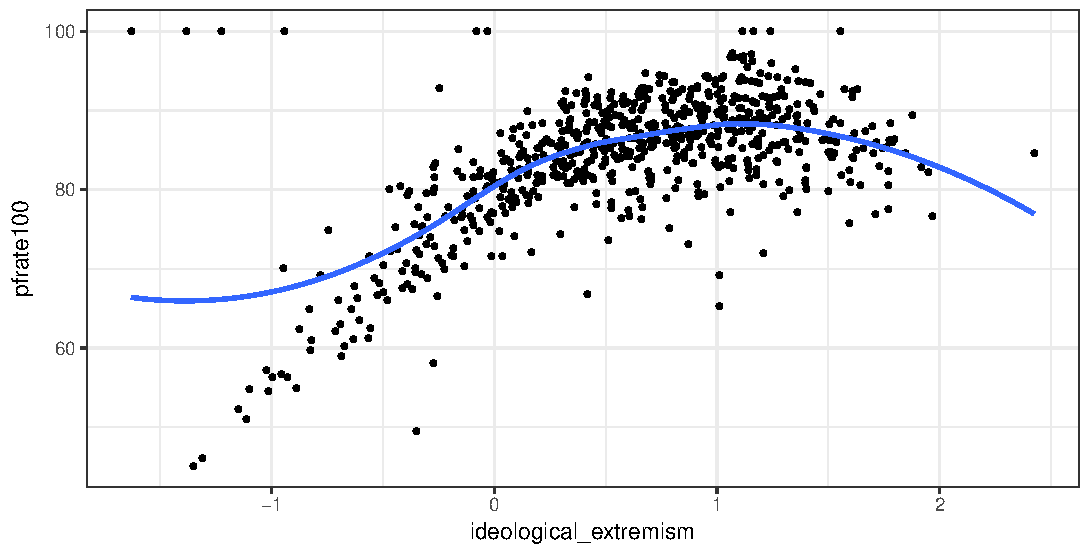
\includegraphics[width = \textwidth]{C:/Users/Ethan/Documents/GitHub/partycalls/plots/senate_iv_iv_dem_maj.pdf}
\end{figure}

\begin{figure}[H]
	\centering
	\caption{Senate DV/IV Plot, Majority Democrats}
	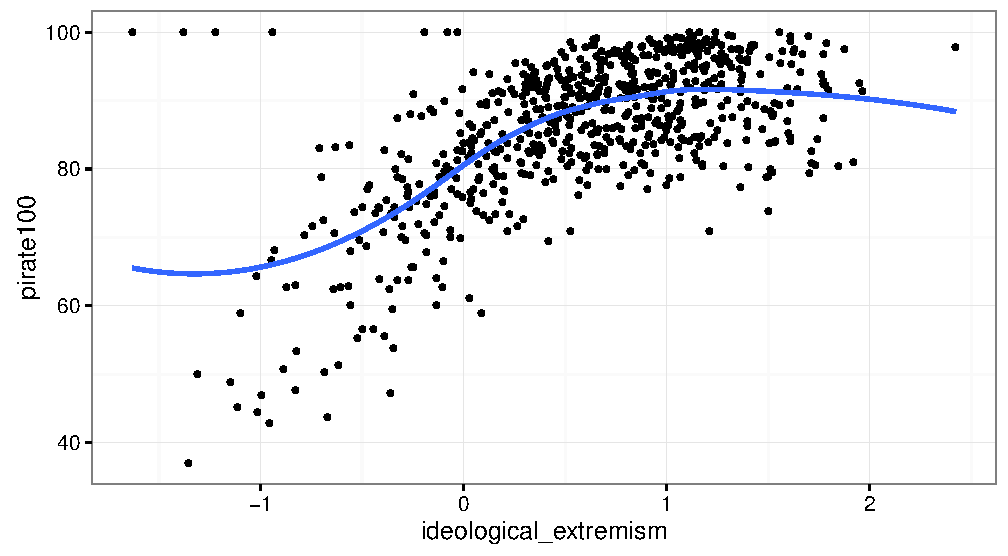
\includegraphics[width = \textwidth]{C:/Users/Ethan/Documents/GitHub/partycalls/plots/senate_iv_dv_dem_maj.pdf}
\end{figure}

\begin{figure}[H]
	\centering
	\caption{Senate IV/IV Plot, Majority Democrats, South/Other}
	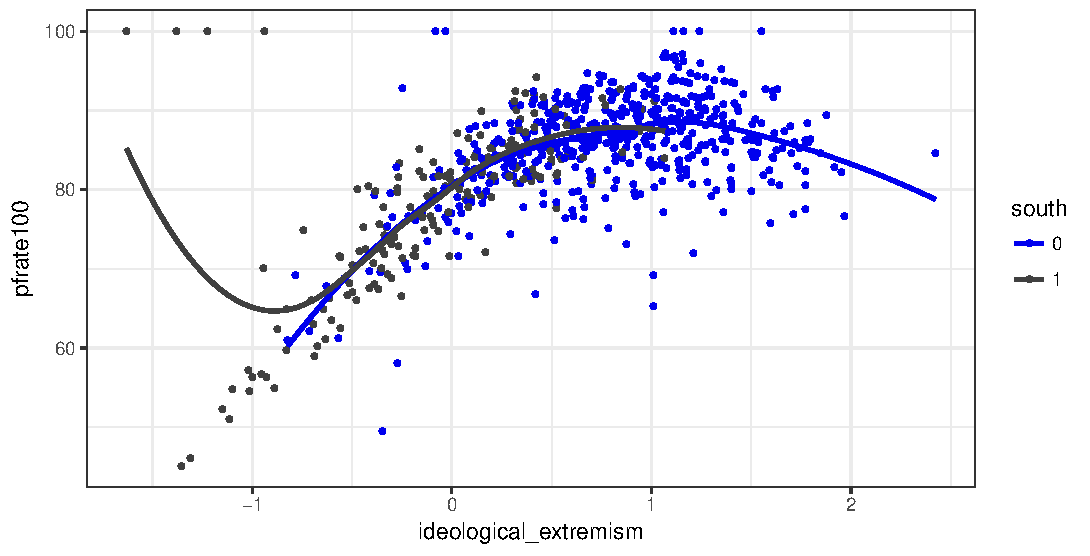
\includegraphics[width = \textwidth]{C:/Users/Ethan/Documents/GitHub/partycalls/plots/senate_iv_iv_dem_maj_south.pdf}
\end{figure}

\begin{figure}[H]
	\centering
	\caption{Senate DV/IV Plot, Majority Democrats, South/Other}
	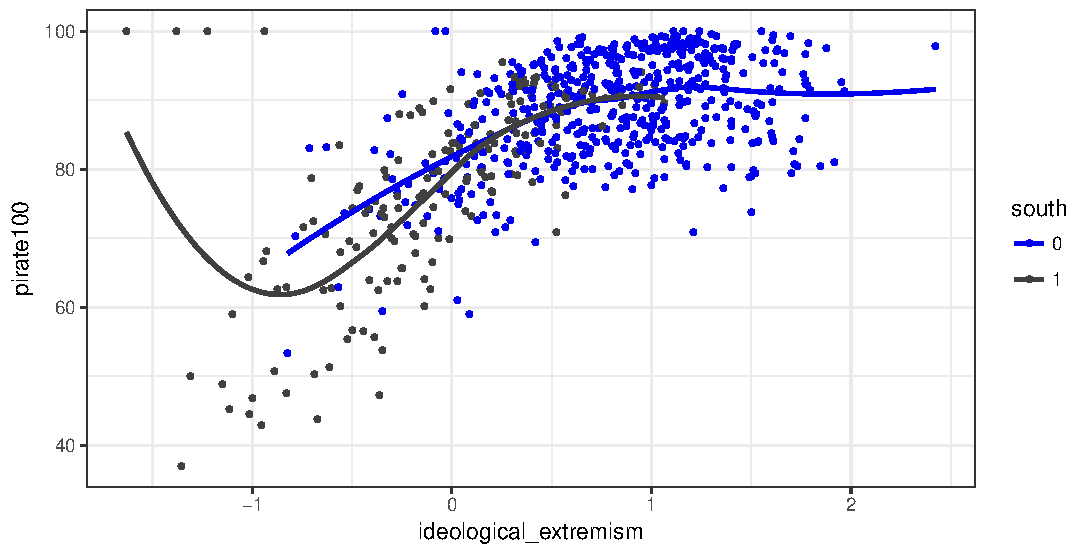
\includegraphics[width = \textwidth]{C:/Users/Ethan/Documents/GitHub/partycalls/plots/senate_iv_dv_dem_maj_south.pdf}
\end{figure}

\begin{figure}[H]
	\centering
	\caption{Senate IV/IV Plot, Minority Democrats}
	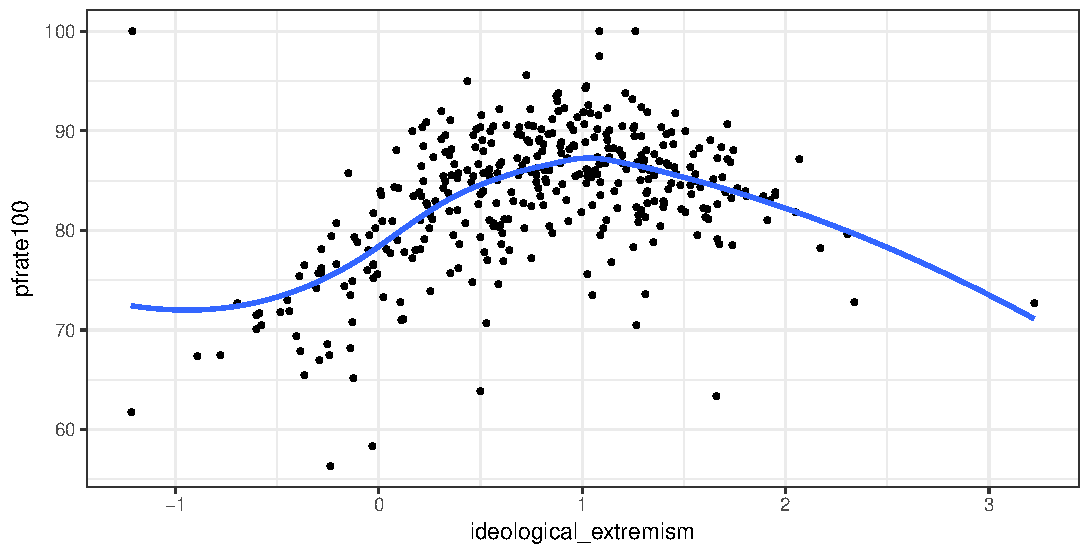
\includegraphics[width = \textwidth]{C:/Users/Ethan/Documents/GitHub/partycalls/plots/senate_iv_iv_dem_min.pdf}
\end{figure}

\begin{figure}[H]
	\centering
	\caption{Senate DV/IV Plot, Minority Democrats}
	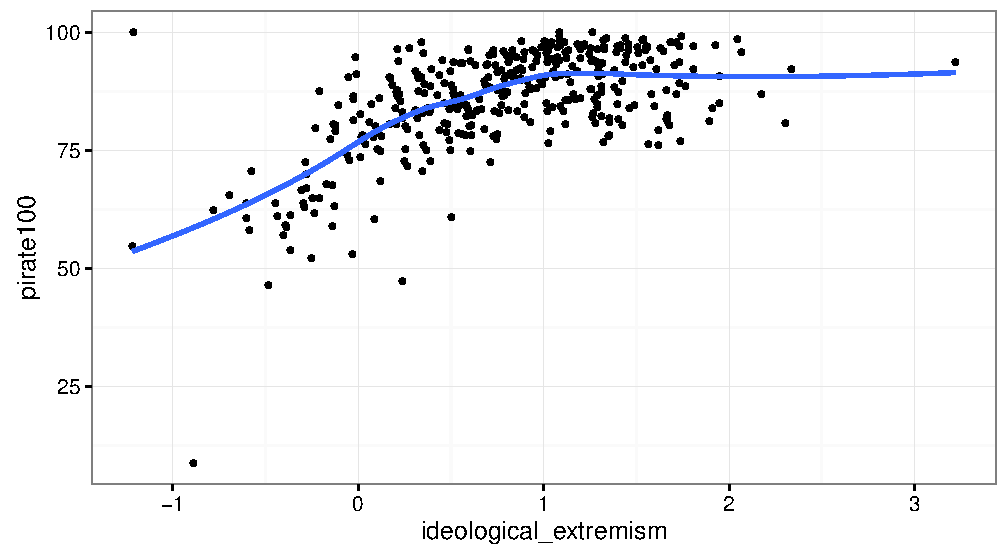
\includegraphics[width = \textwidth]{C:/Users/Ethan/Documents/GitHub/partycalls/plots/senate_iv_dv_dem_min.pdf}
\end{figure}

\begin{figure}[H]
	\centering
	\caption{Senate IV/IV Plot, Minority Democrats, South/Other}
	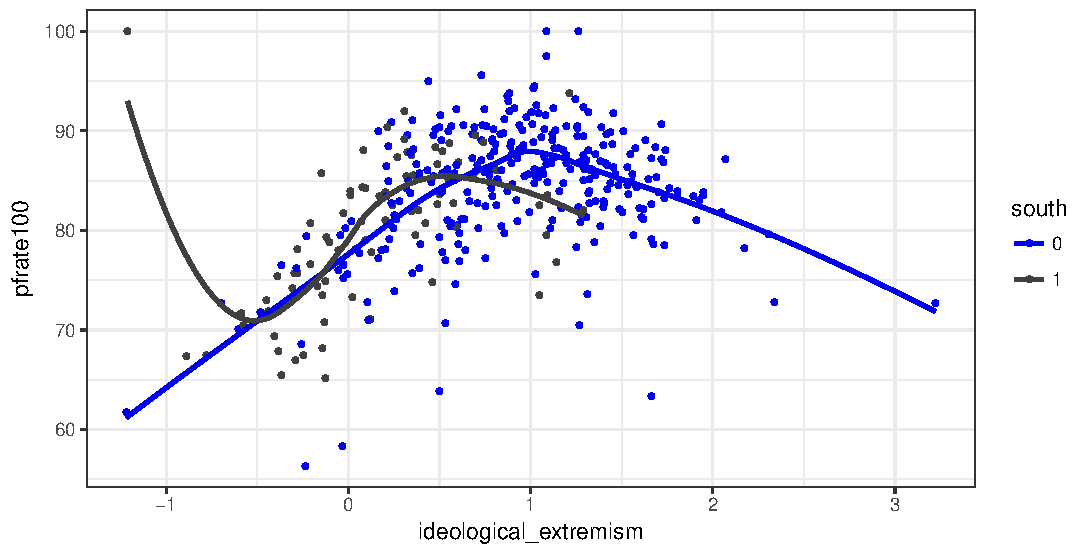
\includegraphics[width = \textwidth]{C:/Users/Ethan/Documents/GitHub/partycalls/plots/senate_iv_iv_dem_min_south.pdf}
\end{figure}

\begin{figure}[H]
	\centering
	\caption{Senate DV/IV Plot, Minority Democrats, South/Other}
	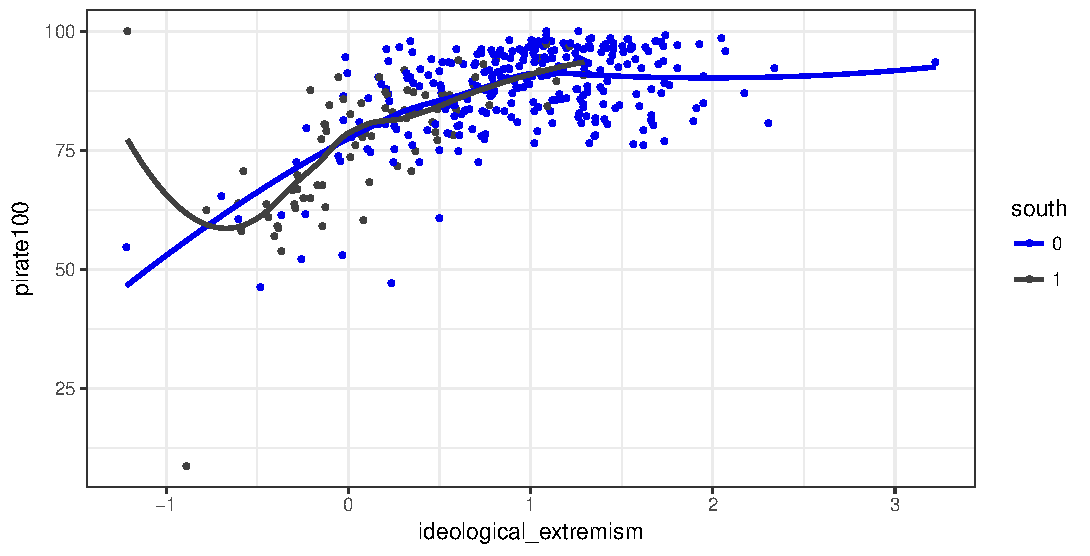
\includegraphics[width = \textwidth]{C:/Users/Ethan/Documents/GitHub/partycalls/plots/senate_iv_dv_dem_min_south.pdf}
\end{figure}

\begin{figure}[H]
	\centering
	\caption{Senate IV/IV Plot, Majority Republicans}
	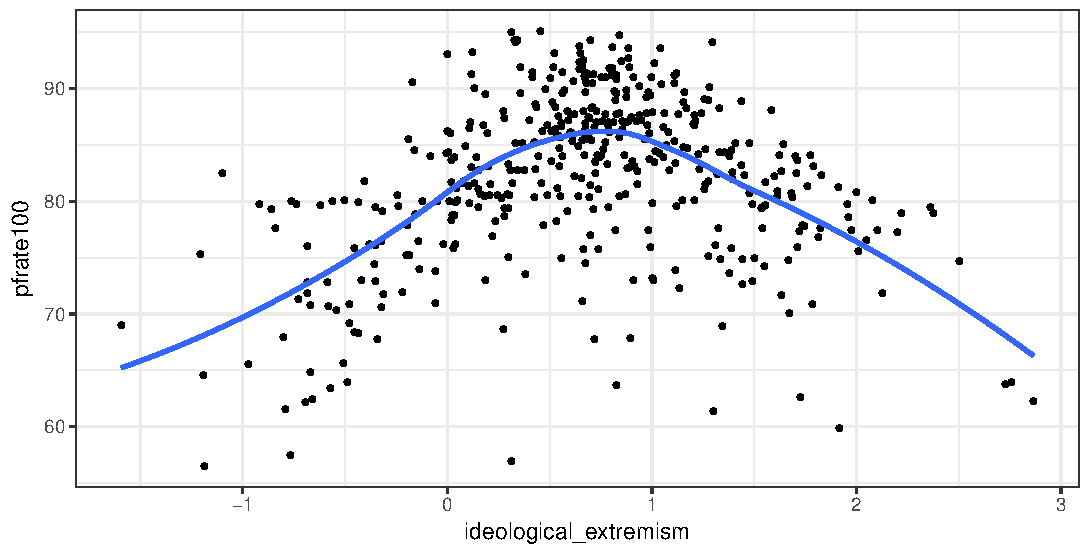
\includegraphics[width = \textwidth]{C:/Users/Ethan/Documents/GitHub/partycalls/plots/senate_iv_iv_rep_maj.pdf}
\end{figure}

\begin{figure}[H]
	\centering
	\caption{Senate DV/IV Plot, Majority Republicans}
	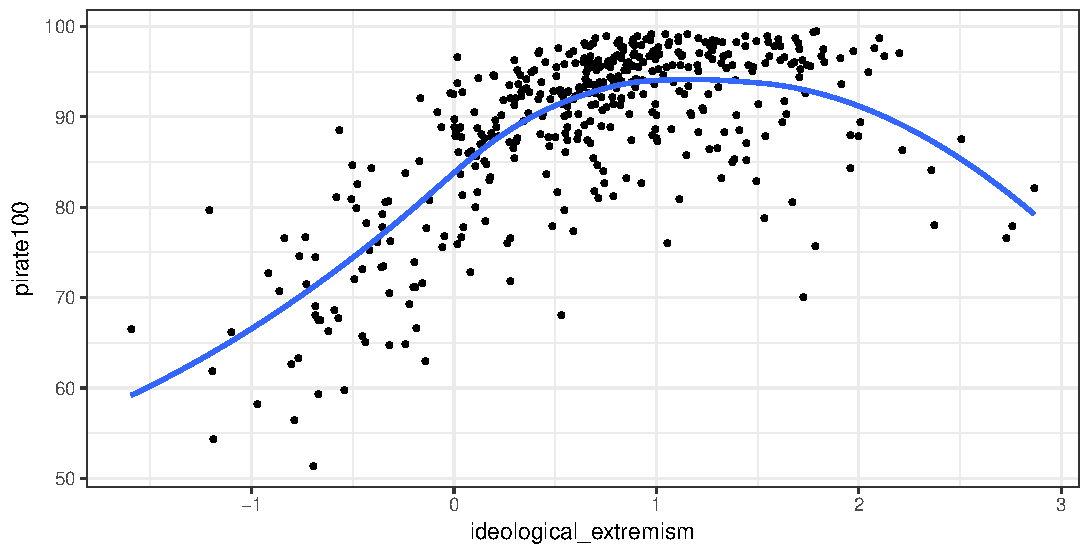
\includegraphics[width = \textwidth]{C:/Users/Ethan/Documents/GitHub/partycalls/plots/senate_iv_dv_rep_maj.pdf}
\end{figure}

\begin{figure}[H]
	\centering
	\caption{Senate IV/IV Plot, Majority Republicans, Gingrich/Other}
	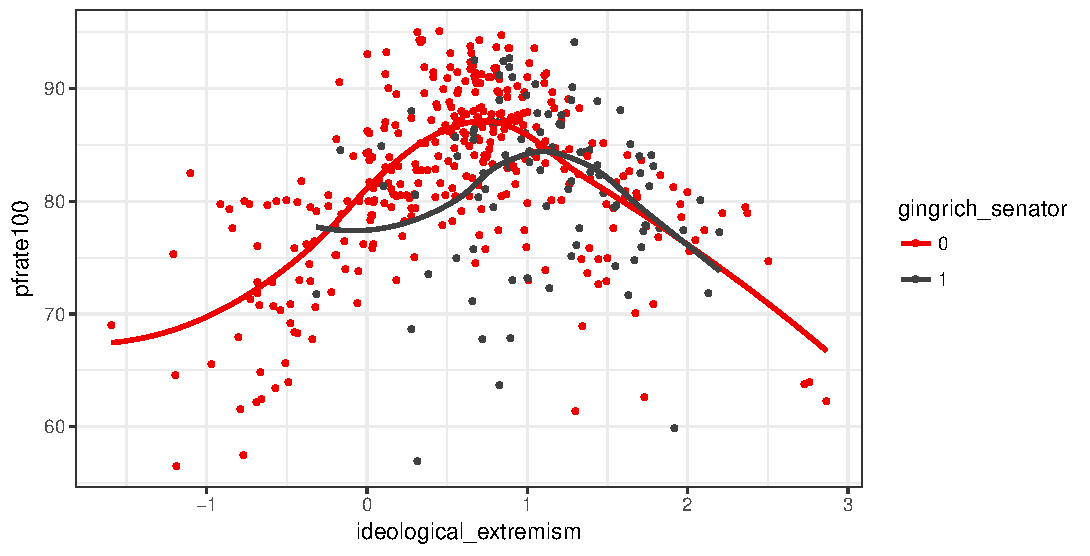
\includegraphics[width = \textwidth]{C:/Users/Ethan/Documents/GitHub/partycalls/plots/senate_iv_iv_rep_maj_gingrich.pdf}
\end{figure}

\begin{figure}[H]
	\centering
	\caption{Senate DV/IV Plot, Majority Republicans, Gingrich/Other}
	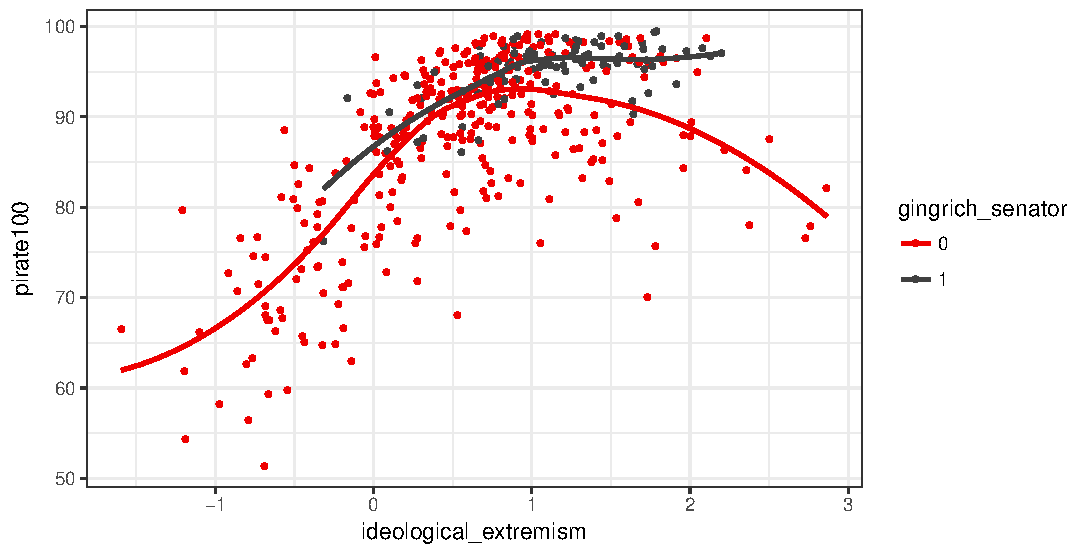
\includegraphics[width = \textwidth]{C:/Users/Ethan/Documents/GitHub/partycalls/plots/senate_iv_dv_rep_maj_gingrich.pdf}
\end{figure}

\begin{figure}[H]
	\centering
	\caption{Senate IV/IV Plot, Minority Republicans}
	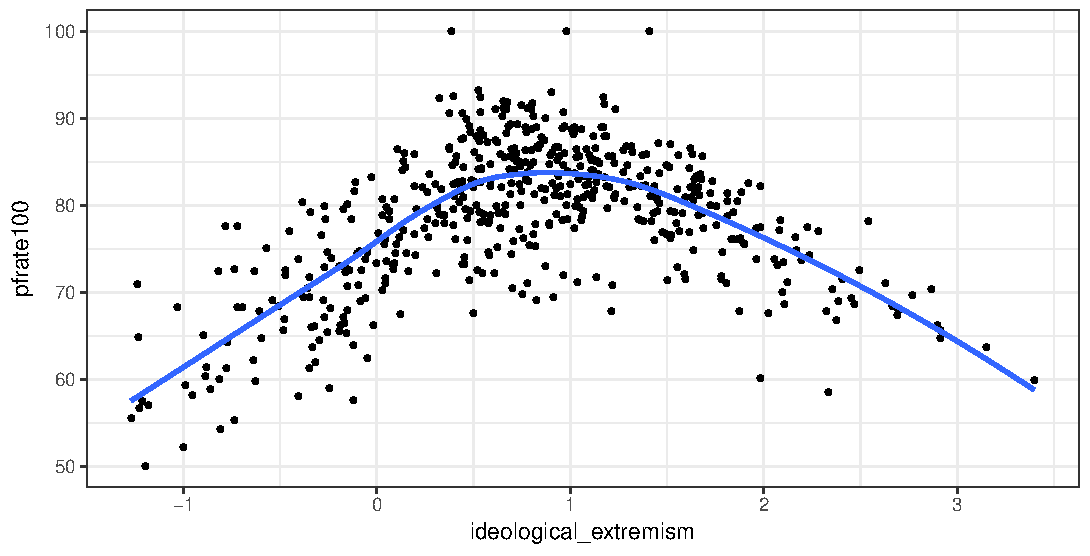
\includegraphics[width = \textwidth]{C:/Users/Ethan/Documents/GitHub/partycalls/plots/senate_iv_iv_rep_min.pdf}
\end{figure}

\begin{figure}[H]
	\centering
	\caption{Senate DV/IV Plot, Minority Republicans}
	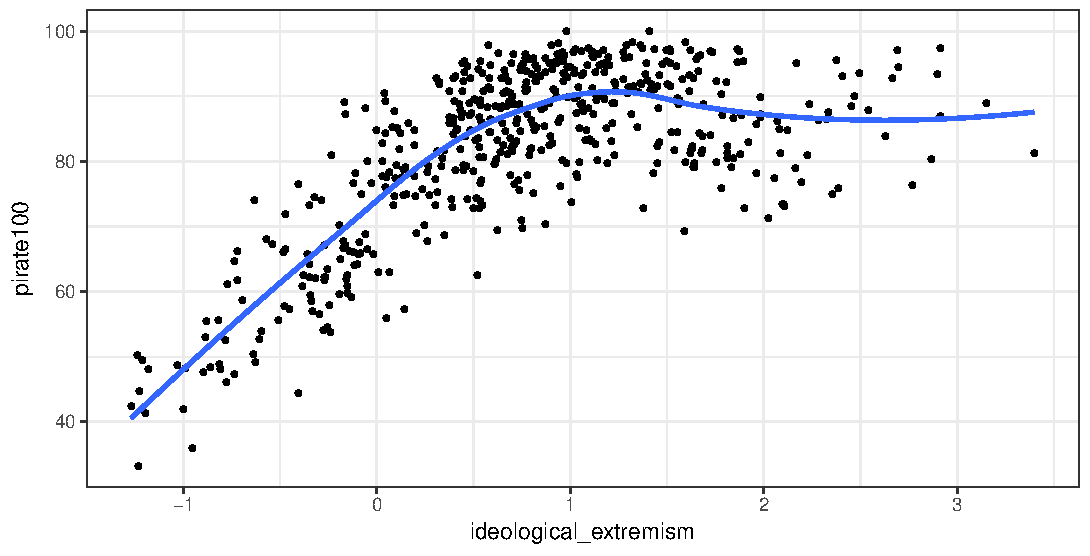
\includegraphics[width = \textwidth]{C:/Users/Ethan/Documents/GitHub/partycalls/plots/senate_iv_dv_rep_min.pdf}
\end{figure}

\begin{figure}[H]
	\centering
	\caption{Senate IV/IV Plot, Minority Republicans, Gingrich/Other}
	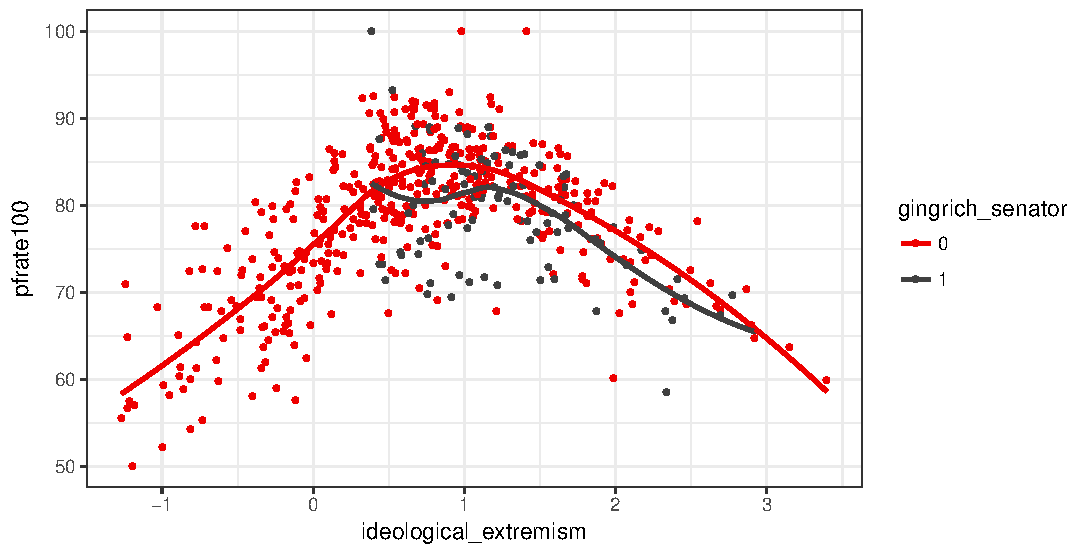
\includegraphics[width = \textwidth]{C:/Users/Ethan/Documents/GitHub/partycalls/plots/senate_iv_iv_rep_min_gingrich.pdf}
\end{figure}

\begin{figure}[H]
	\centering
	\caption{Senate DV/IV Plot, Minority Republicans, Gingrich/Other}
	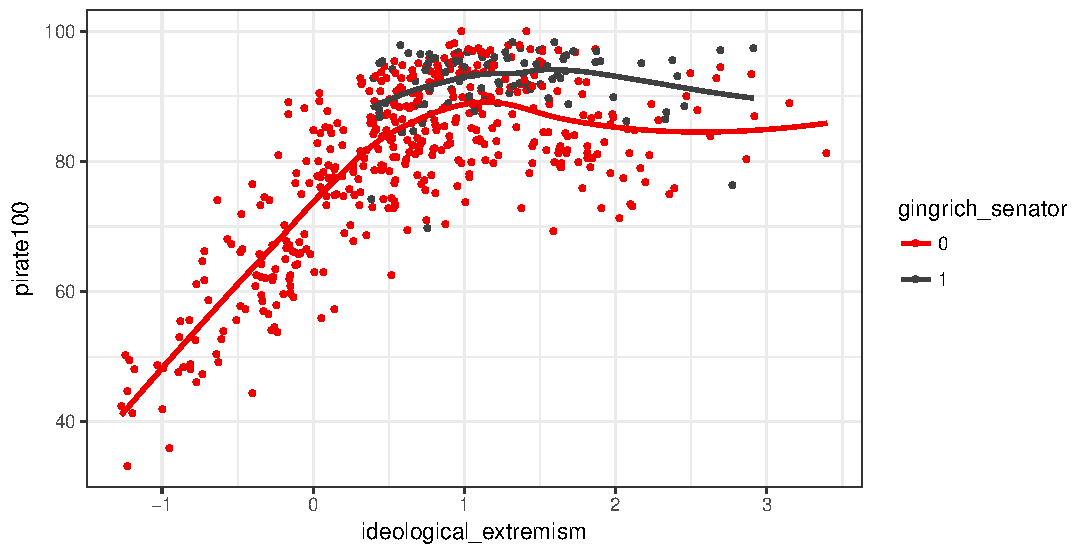
\includegraphics[width = \textwidth]{C:/Users/Ethan/Documents/GitHub/partycalls/plots/senate_iv_dv_rep_min_gingrich.pdf}
\end{figure}

\begin{figure}[H]
	\centering
	\caption{House IV/IV Plot, Majority Democrats}
	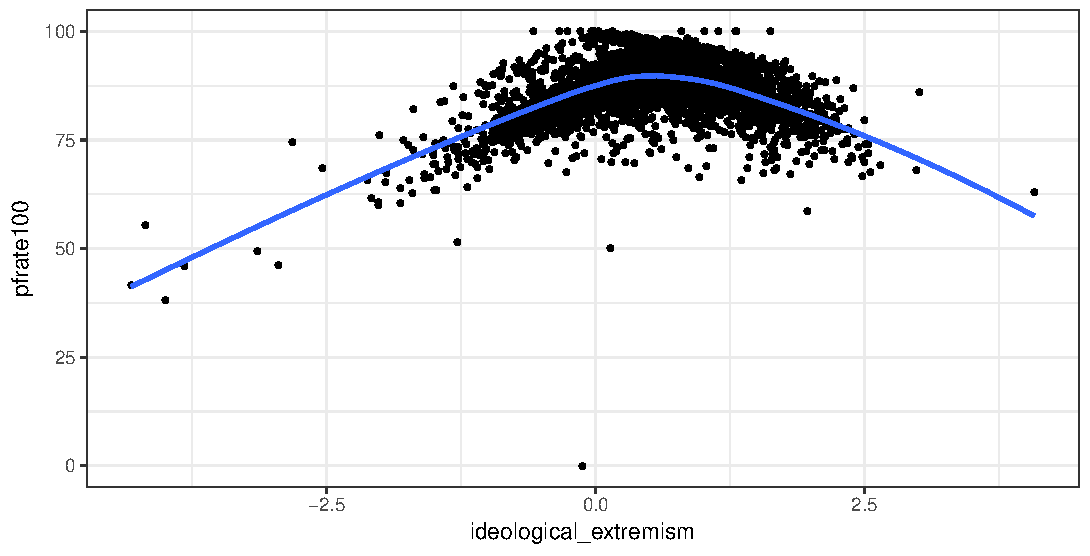
\includegraphics[width = \textwidth]{C:/Users/Ethan/Documents/GitHub/partycalls/plots/house_iv_iv_dem_maj.pdf}
\end{figure}

\begin{figure}[H]
	\centering
	\caption{House DV/IV Plot, Majority Democrats}
	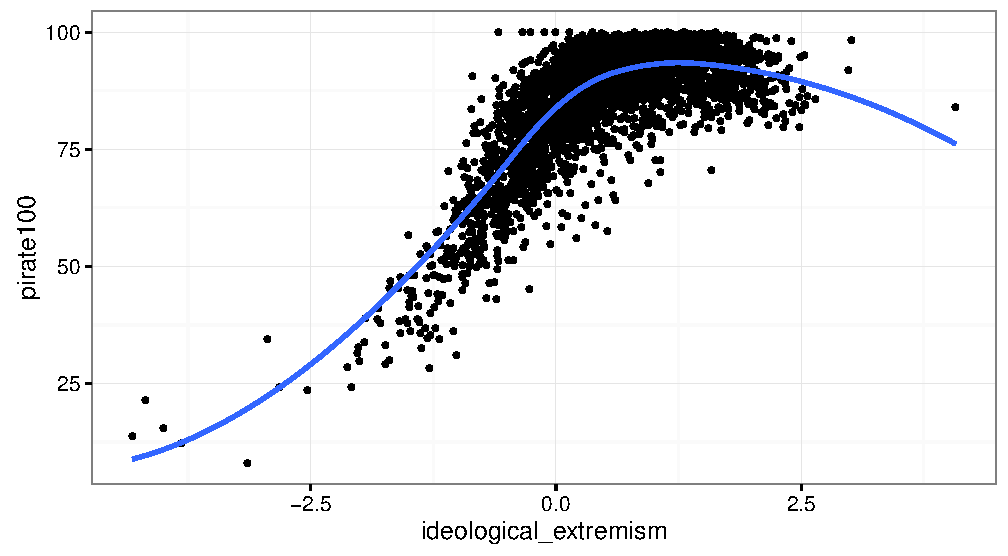
\includegraphics[width = \textwidth]{C:/Users/Ethan/Documents/GitHub/partycalls/plots/house_iv_dv_dem_maj.pdf}
\end{figure}

\begin{figure}[H]
	\centering
	\caption{House IV/IV Plot, Majority Democrats, South/Other}
	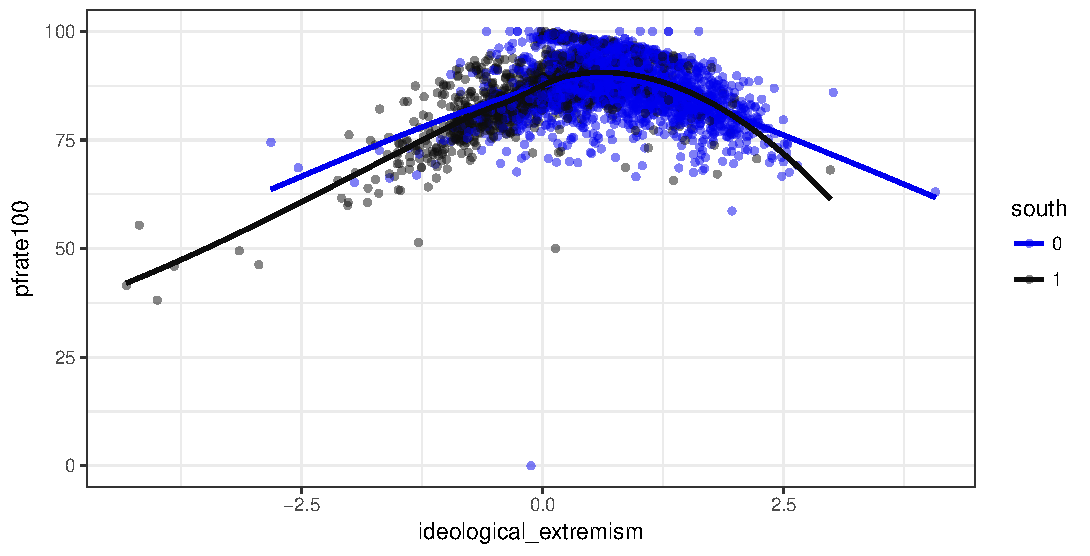
\includegraphics[width = \textwidth]{C:/Users/Ethan/Documents/GitHub/partycalls/plots/house_iv_iv_dem_maj_south.pdf}
\end{figure}

\begin{figure}[H]
	\centering
	\caption{House DV/IV Plot, Majority Democrats, South/Other}
	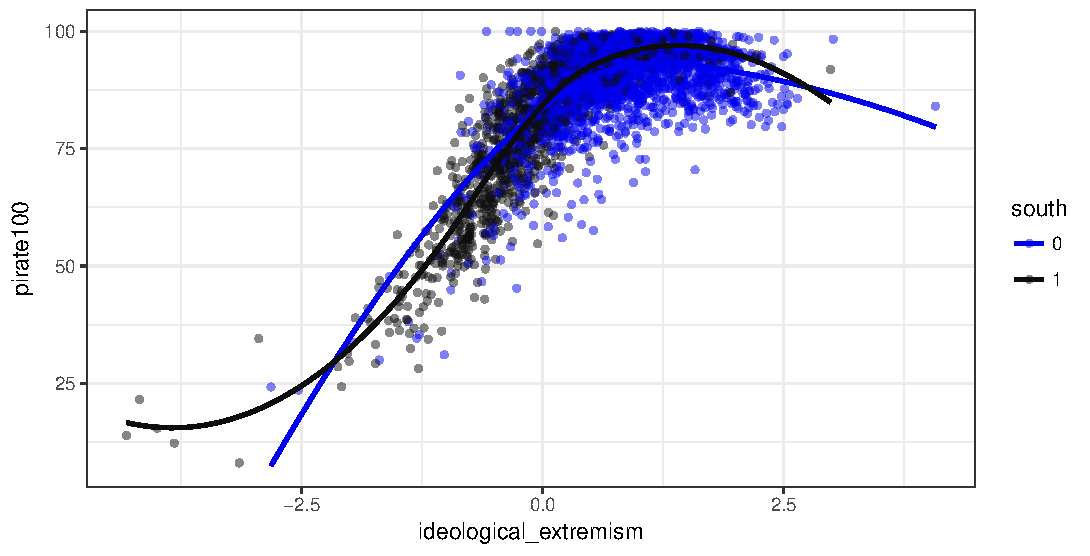
\includegraphics[width = \textwidth]{C:/Users/Ethan/Documents/GitHub/partycalls/plots/house_iv_dv_dem_maj_south.pdf}
\end{figure}

\begin{figure}[H]
	\centering
	\caption{House IV/IV Plot, Minority Democrats}
	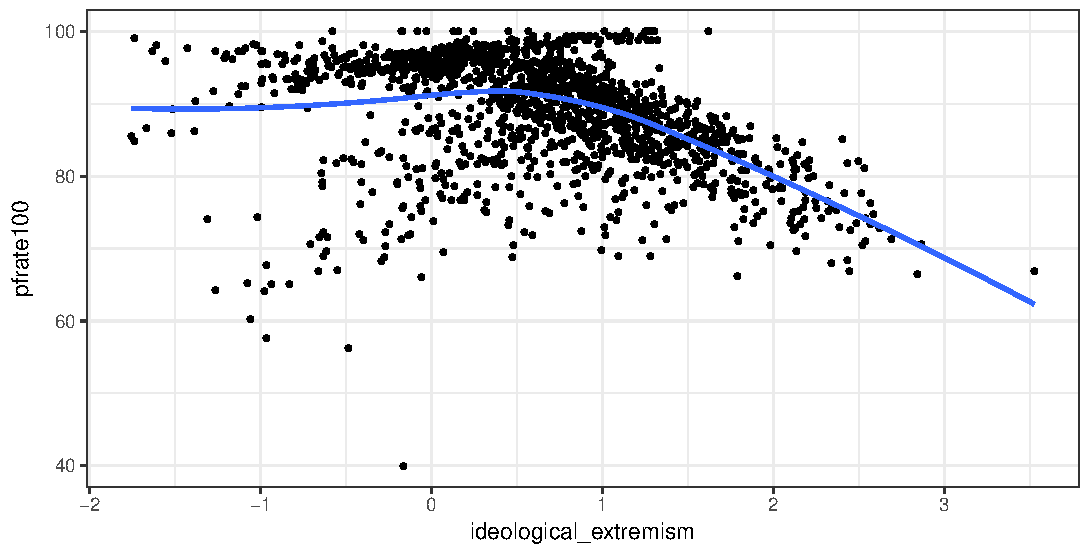
\includegraphics[width = \textwidth]{C:/Users/Ethan/Documents/GitHub/partycalls/plots/house_iv_iv_dem_min.pdf}
\end{figure}

\begin{figure}[H]
	\centering
	\caption{House DV/IV Plot, Minority Democrats}
	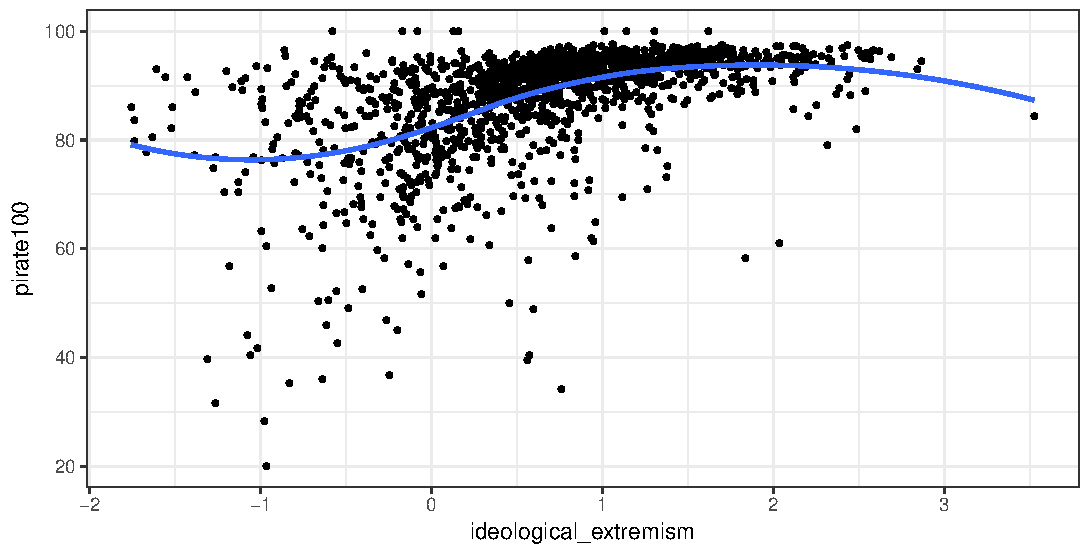
\includegraphics[width = \textwidth]{C:/Users/Ethan/Documents/GitHub/partycalls/plots/house_iv_dv_dem_min.pdf}
\end{figure}

\begin{figure}[H]
	\centering
	\caption{House IV/IV Plot, Minority Democrats, South/Other}
	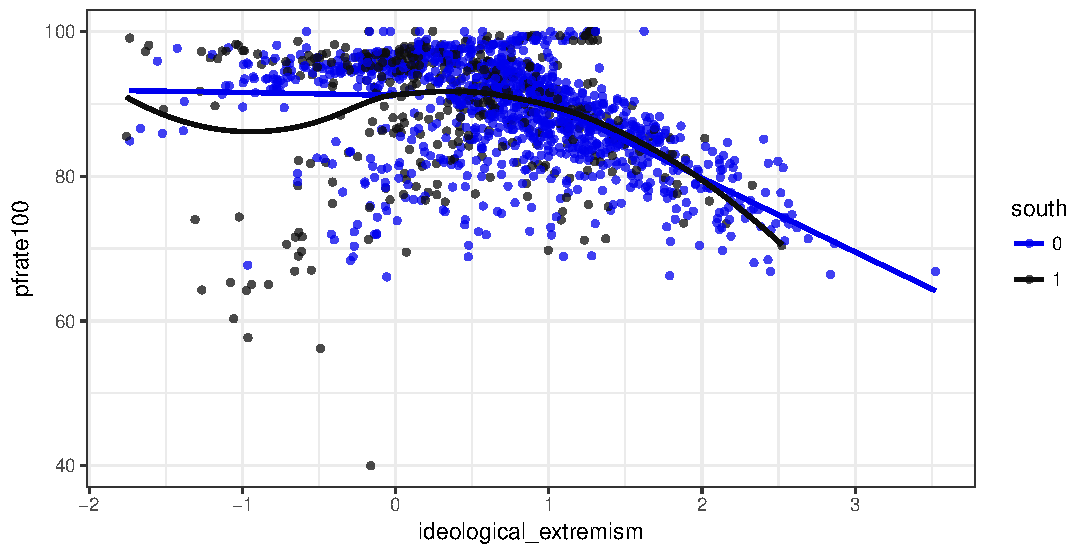
\includegraphics[width = \textwidth]{C:/Users/Ethan/Documents/GitHub/partycalls/plots/house_iv_iv_dem_min_south.pdf}
\end{figure}

\begin{figure}[H]
	\centering
	\caption{House DV/IV Plot, Minority Democrats, South/Other}
	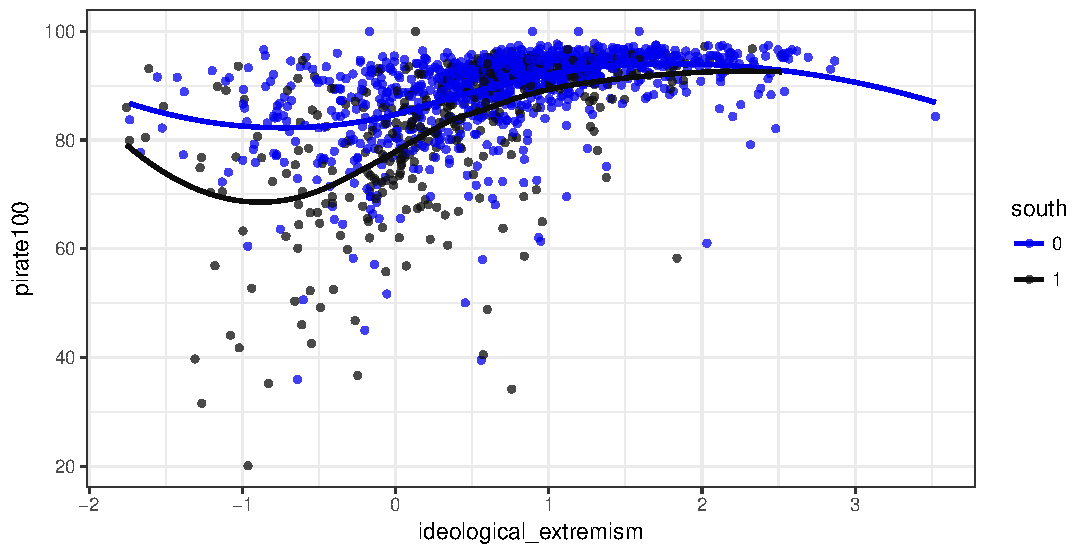
\includegraphics[width = \textwidth]{C:/Users/Ethan/Documents/GitHub/partycalls/plots/house_iv_dv_dem_min_south.pdf}
\end{figure}

\begin{figure}[H]
	\centering
	\caption{House IV/IV Plot, Majority Republicans}
	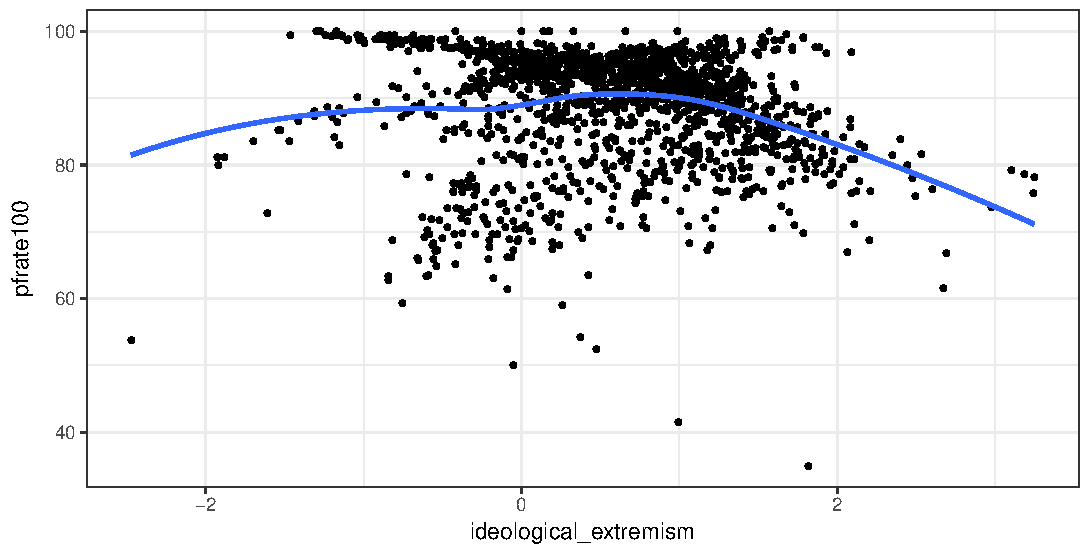
\includegraphics[width = \textwidth]{C:/Users/Ethan/Documents/GitHub/partycalls/plots/house_iv_iv_rep_maj.pdf}
\end{figure}

\begin{figure}[H]
	\centering
	\caption{House DV/IV Plot, Majority Republicans}
	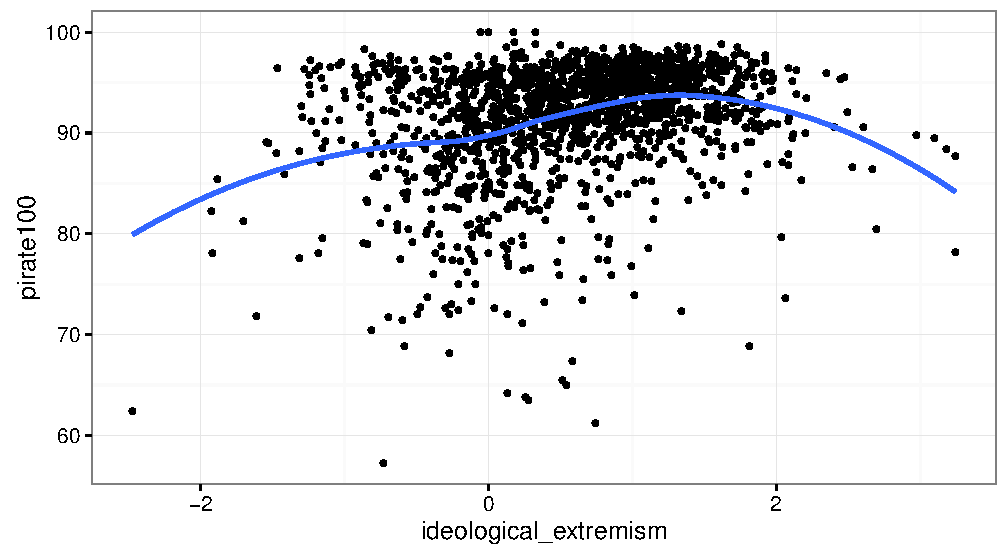
\includegraphics[width = \textwidth]{C:/Users/Ethan/Documents/GitHub/partycalls/plots/house_iv_dv_rep_maj.pdf}
\end{figure}

\begin{figure}[H]
	\centering
	\caption{House IV/IV Plot, Minority Republicans}
	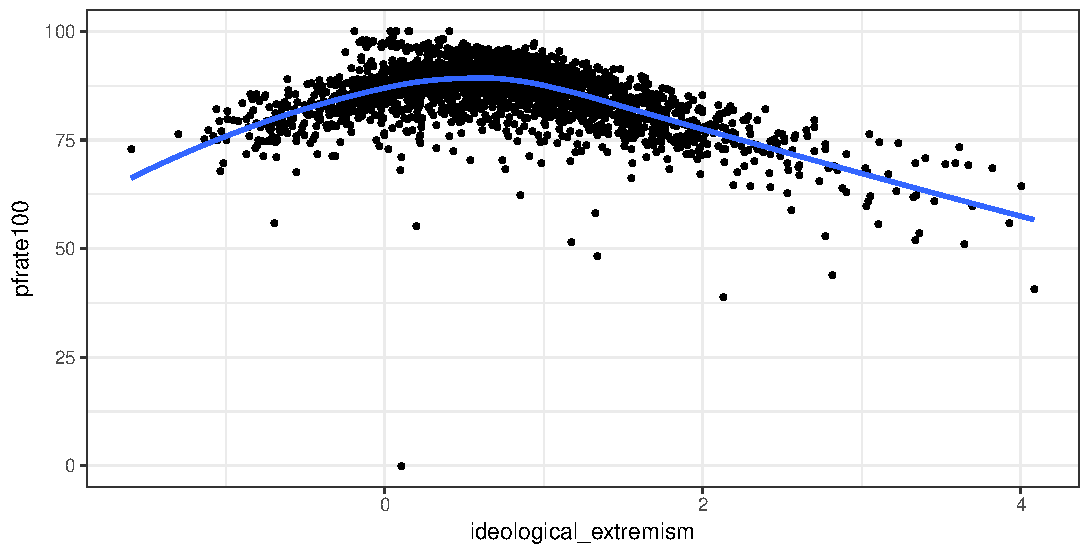
\includegraphics[width = \textwidth]{C:/Users/Ethan/Documents/GitHub/partycalls/plots/house_iv_iv_rep_min.pdf}
\end{figure}


\begin{figure}[H]
	\centering
	\caption{House DV/IV Plot, Minority Republicans}
	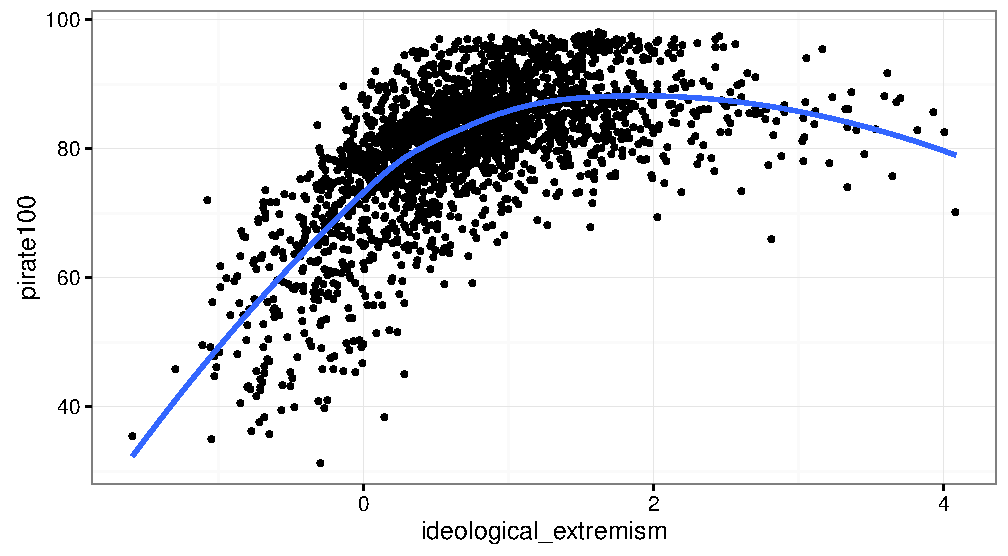
\includegraphics[width = \textwidth]{C:/Users/Ethan/Documents/GitHub/partycalls/plots/house_iv_dv_rep_min.pdf}
\end{figure}



\clearpage

\subsection{Variable Checks}

\begin{figure}[H]
\centering
\caption{Presidential Vote Share and Democratic Presidential Vote Share: All}
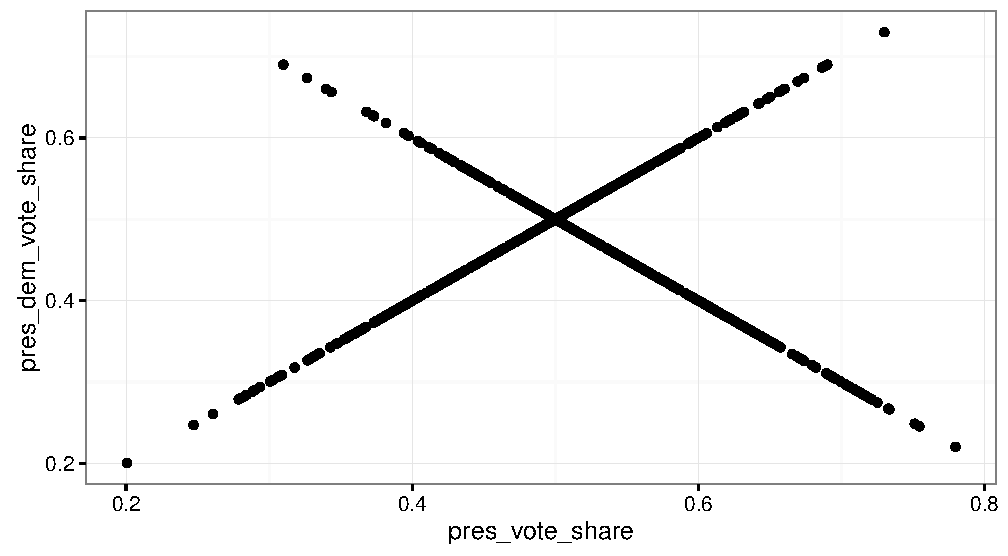
\includegraphics[width = \textwidth]{C:/Users/Ethan/Documents/GitHub/partycalls/plots/pres_vote_check_all.pdf}
\end{figure}

\begin{figure}[H]
	\centering
	\caption{Presidential Vote Share and Democratic Presidential Vote Share: Democrats}
	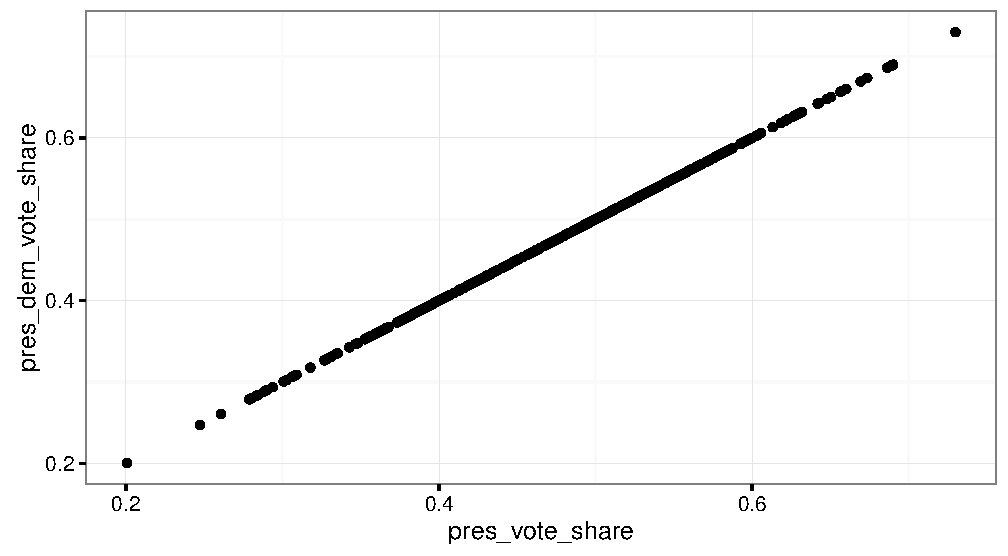
\includegraphics[width = \textwidth]{C:/Users/Ethan/Documents/GitHub/partycalls/plots/pres_vote_check_dem.pdf}
\end{figure}

\begin{figure}[H]
	\centering
	\caption{Presidential Vote Share and Democratic Presidential Vote Share: Republicans}
	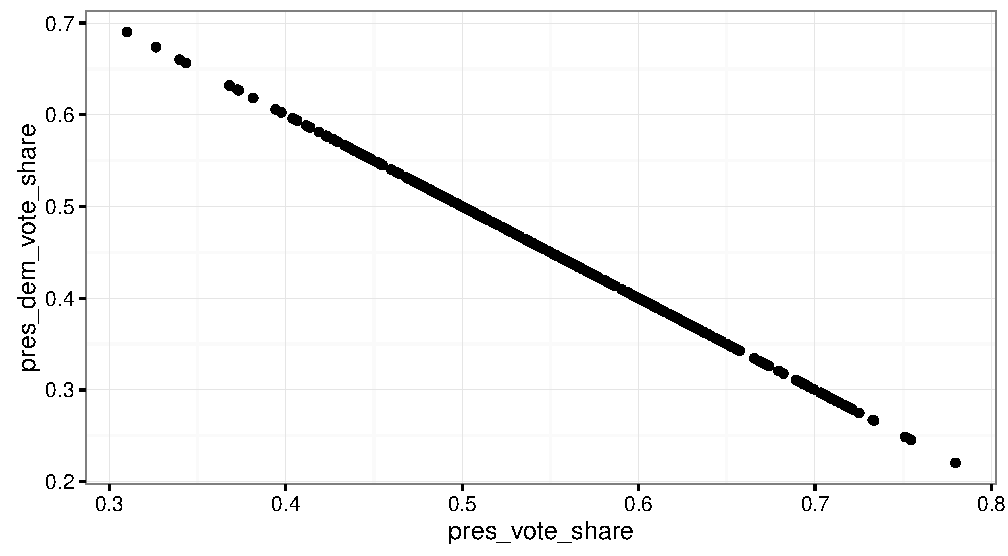
\includegraphics[width = \textwidth]{C:/Users/Ethan/Documents/GitHub/partycalls/plots/pres_vote_check_rep.pdf}
\end{figure}

\clearpage

\section{Past Tables and Figures to Include in Paper}

\subsection{Senate}

% Table created by stargazer v.5.2 by Marek Hlavac, Harvard University. E-mail: hlavac at fas.harvard.edu
% Date and time: Mon, Mar 06, 2017 - 11:46:30
\begin{table}[H] \centering 
	\caption{Senate Variable Summaries} 
	\label{} 
	\begin{tabular}{@{\extracolsep{5pt}}lccccc} 
		\\[-1.8ex]\hline 
		\hline \\[-1.8ex] 
		Statistic & \multicolumn{1}{c}{N} & \multicolumn{1}{c}{Mean} & \multicolumn{1}{c}{St. Dev.} & \multicolumn{1}{c}{Min} & \multicolumn{1}{c}{Max} \\ 
		\hline \\[-1.8ex] 
		congress & 1,993 & 102.511 & 5.771 & 93 & 112 \\ 
		icpsrLegis & 1,993 & 18,808.510 & 13,984.900 & 52 & 95,407 \\ 
		class & 1,993 & 2.012 & 0.819 & 1 & 3 \\ 
		maj & 1,993 & 0.552 & 0.488 & 0.000 & 1.000 \\ 
		pres\_vote\_share & 1,993 & 0.521 & 0.097 & 0.201 & 0.780 \\ 
		pres\_dem\_vote\_share & 1,993 & 0.462 & 0.092 & 0.201 & 0.730 \\ 
		vote\_share & 1,993 & 0.612 & 0.099 & 0.500 & 1.000 \\ 
		south & 1,993 & 0.260 & 0.439 & 0 & 1 \\ 
		south11 & 1,993 & 0.220 & 0.414 & 0 & 1 \\ 
		south13 & 1,993 & 0.260 & 0.439 & 0 & 1 \\ 
		south17 & 1,993 & 0.339 & 0.473 & 0 & 1 \\ 
		south\_dem & 1,993 & 0.123 & 0.329 & 0 & 1 \\ 
		leader & 1,993 & 0.099 & 0.299 & 0 & 1 \\ 
		chair & 1,993 & 0.183 & 0.386 & 0 & 1 \\ 
		best\_committee & 1,993 & 12.277 & 2.740 & 0 & 15 \\ 
		power\_committee & 1,993 & 0.727 & 0.446 & 0 & 1 \\ 
		up\_for\_reelection & 1,993 & 0.333 & 0.471 & 0 & 1 \\ 
		freshman & 1,993 & 0.114 & 0.318 & 0 & 1 \\ 
		superfreshman & 1,993 & 0.003 & 0.050 & 0 & 1 \\ 
		seniority & 1,993 & 6.254 & 4.618 & 1 & 26 \\ 
		senate\_seniority & 1,993 & 2.424 & 1.527 & 1 & 9 \\ 
		retiree & 1,993 & 0.059 & 0.235 & 0 & 1 \\ 
		first\_term & 1,993 & 0.356 & 0.479 & 0 & 1 \\ 
		afam & 1,993 & 0.004 & 0.063 & 0 & 1 \\ 
		female & 1,993 & 0.067 & 0.250 & 0 & 1 \\ 
		latino & 1,993 & 0.008 & 0.086 & 0 & 1 \\ 
		gingrich\_senator & 1,993 & 0.094 & 0.292 & 0 & 1 \\ 
		votes & 1,993 & 733.147 & 199.048 & 5 & 1,311 \\ 
		drop & 1,993 & 0.000 & 0.000 & 0 & 0 \\ 
		party\_free\_ideal\_point & 1,993 & 0.002 & 1.000 & $-$3.222 & 3.397 \\ 
		pirate100 & 1,993 & 85.491 & 11.438 & 8.777 & 100.000 \\ 
		pfrate100 & 1,993 & 82.035 & 8.164 & 45.106 & 100.000 \\ 
		ideological\_extremism & 1,993 & 0.689 & 0.724 & $-$1.630 & 3.397 \\
		\hline \\[-1.8ex] 
	\end{tabular} 
\end{table} 

% Table created by stargazer v.5.2 by Marek Hlavac, Harvard University. E-mail: hlavac at fas.harvard.edu
% Date and time: Mon, Mar 06, 2017 - 12:25:53
\begin{table}[H] \centering 
	\caption{Senate Variable Summaries, Democrats} 
	\label{} 
	\begin{tabular}{@{\extracolsep{5pt}}lccccc} 
		\\[-1.8ex]\hline 
		\hline \\[-1.8ex] 
		Statistic & \multicolumn{1}{c}{N} & \multicolumn{1}{c}{Mean} & \multicolumn{1}{c}{St. Dev.} & \multicolumn{1}{c}{Min} & \multicolumn{1}{c}{Max} \\ 
		\hline \\[-1.8ex] 
		congress & 1,042 & 102.262 & 5.886 & 93 & 112 \\ 
		icpsrLegis & 1,042 & 17,125.290 & 12,528.160 & 660 & 94,910 \\ 
		class & 1,042 & 1.964 & 0.844 & 1 & 3 \\ 
		maj & 1,042 & 0.633 & 0.473 & 0.000 & 1.000 \\ 
		pres\_vote\_share & 1,042 & 0.484 & 0.093 & 0.201 & 0.730 \\ 
		pres\_dem\_vote\_share & 1,042 & 0.484 & 0.093 & 0.201 & 0.730 \\ 
		vote\_share & 1,042 & 0.619 & 0.102 & 0.500 & 1.000 \\ 
		south & 1,042 & 0.236 & 0.425 & 0 & 1 \\ 
		south11 & 1,042 & 0.211 & 0.408 & 0 & 1 \\ 
		south13 & 1,042 & 0.236 & 0.425 & 0 & 1 \\ 
		south17 & 1,042 & 0.340 & 0.474 & 0 & 1 \\ 
		south\_dem & 1,042 & 0.236 & 0.425 & 0 & 1 \\ 
		leader & 1,042 & 0.083 & 0.277 & 0 & 1 \\ 
		chair & 1,042 & 0.208 & 0.406 & 0 & 1 \\ 
		best\_committee & 1,042 & 12.257 & 2.780 & 0 & 15 \\ 
		power\_committee & 1,042 & 0.729 & 0.445 & 0 & 1 \\ 
		up\_for\_reelection & 1,042 & 0.334 & 0.472 & 0 & 1 \\ 
		freshman & 1,042 & 0.105 & 0.306 & 0 & 1 \\ 
		superfreshman & 1,042 & 0.003 & 0.054 & 0 & 1 \\ 
		seniority & 1,042 & 6.781 & 4.940 & 1 & 26 \\ 
		senate\_seniority & 1,042 & 2.597 & 1.636 & 1 & 9 \\ 
		retiree & 1,042 & 0.051 & 0.220 & 0 & 1 \\ 
		first\_term & 1,042 & 0.328 & 0.470 & 0 & 1 \\ 
		afam & 1,042 & 0.005 & 0.069 & 0 & 1 \\ 
		female & 1,042 & 0.084 & 0.278 & 0 & 1 \\ 
		latino & 1,042 & 0.008 & 0.087 & 0 & 1 \\ 
		gingrich\_senator & 1,042 & 0.000 & 0.000 & 0 & 0 \\ 
		votes & 1,042 & 740.120 & 208.038 & 5 & 1,311 \\ 
		drop & 1,042 & 0.000 & 0.000 & 0 & 0 \\ 
		party\_free\_ideal\_point & 1,042 & $-$0.657 & 0.657 & $-$3.222 & 1.630 \\ 
		pirate100 & 1,042 & 85.776 & 10.886 & 8.777 & 100.000 \\ 
		pfrate100 & 1,042 & 83.760 & 7.862 & 45.106 & 100.000 \\ 
		ideological\_extremism & 1,042 & 0.657 & 0.657 & $-$1.630 & 3.222 \\ 
		\hline \\[-1.8ex] 
	\end{tabular} 
\end{table} 

% Table created by stargazer v.5.2 by Marek Hlavac, Harvard University. E-mail: hlavac at fas.harvard.edu
% Date and time: Mon, Mar 06, 2017 - 12:25:56
\begin{table}[H] \centering 
	\caption{Senate Variable Summaries, Republicans} 
	\label{} 
	\begin{tabular}{@{\extracolsep{5pt}}lccccc} 
		\\[-1.8ex]\hline 
		\hline \\[-1.8ex] 
		Statistic & \multicolumn{1}{c}{N} & \multicolumn{1}{c}{Mean} & \multicolumn{1}{c}{St. Dev.} & \multicolumn{1}{c}{Min} & \multicolumn{1}{c}{Max} \\ 
		\hline \\[-1.8ex] 
		congress & 951 & 102.784 & 5.633 & 93 & 112 \\ 
		icpsrLegis & 951 & 20,652.800 & 15,218.180 & 52 & 95,407 \\ 
		class & 951 & 2.064 & 0.787 & 1 & 3 \\ 
		maj & 951 & 0.464 & 0.489 & 0.000 & 1.000 \\ 
		pres\_vote\_share & 951 & 0.562 & 0.085 & 0.310 & 0.780 \\ 
		pres\_dem\_vote\_share & 951 & 0.438 & 0.085 & 0.220 & 0.690 \\ 
		vote\_share & 951 & 0.605 & 0.094 & 0.500 & 1.000 \\ 
		south & 951 & 0.286 & 0.452 & 0 & 1 \\ 
		south11 & 951 & 0.229 & 0.421 & 0 & 1 \\ 
		south13 & 951 & 0.286 & 0.452 & 0 & 1 \\ 
		south17 & 951 & 0.338 & 0.473 & 0 & 1 \\ 
		south\_dem & 951 & 0.000 & 0.000 & 0 & 0 \\ 
		leader & 951 & 0.117 & 0.321 & 0 & 1 \\ 
		chair & 951 & 0.155 & 0.362 & 0 & 1 \\ 
		best\_committee & 951 & 12.300 & 2.697 & 0 & 15 \\ 
		power\_committee & 951 & 0.723 & 0.448 & 0 & 1 \\ 
		up\_for\_reelection & 951 & 0.332 & 0.471 & 0 & 1 \\ 
		freshman & 951 & 0.124 & 0.330 & 0 & 1 \\ 
		superfreshman & 951 & 0.002 & 0.046 & 0 & 1 \\ 
		seniority & 951 & 5.677 & 4.163 & 1 & 24 \\ 
		senate\_seniority & 951 & 2.234 & 1.373 & 1 & 8 \\ 
		retiree & 951 & 0.067 & 0.251 & 0 & 1 \\ 
		first\_term & 951 & 0.386 & 0.487 & 0 & 1 \\ 
		afam & 951 & 0.003 & 0.056 & 0 & 1 \\ 
		female & 951 & 0.048 & 0.215 & 0 & 1 \\ 
		latino & 951 & 0.007 & 0.086 & 0 & 1 \\ 
		gingrich\_senator & 951 & 0.198 & 0.398 & 0 & 1 \\ 
		votes & 951 & 725.506 & 188.520 & 40 & 1,291 \\ 
		drop & 951 & 0.000 & 0.000 & 0 & 0 \\ 
		party\_free\_ideal\_point & 951 & 0.725 & 0.789 & $-$1.595 & 3.397 \\ 
		pirate100 & 951 & 85.180 & 12.011 & 33.232 & 100.000 \\ 
		pfrate100 & 951 & 80.144 & 8.073 & 50.070 & 100.000 \\ 
		ideological\_extremism & 951 & 0.725 & 0.789 & $-$1.595 & 3.397 \\ 
		\hline \\[-1.8ex] 
	\end{tabular} 
\end{table} 

% latex table generated in R 3.3.2 by xtable 1.8-2 package
% Thu Feb 23 17:23:31 2017
\begin{table}[H]
	\centering
	\caption{Senate Sorting Algorithm Coefficient Signs}
	\begin{tabular}{rrr}
		\hline
		& ($-$) Ideal & (+) Ideal \\ 
		\hline
		($-$) Party & 0.33 & 0.16 \\ 
		(+) Party & 0.23 & 0.28 \\ 
		\hline
	\end{tabular}
\end{table}

\begin{figure}[H]
	\centering
	\caption{Senate Party Calls by Congress}
	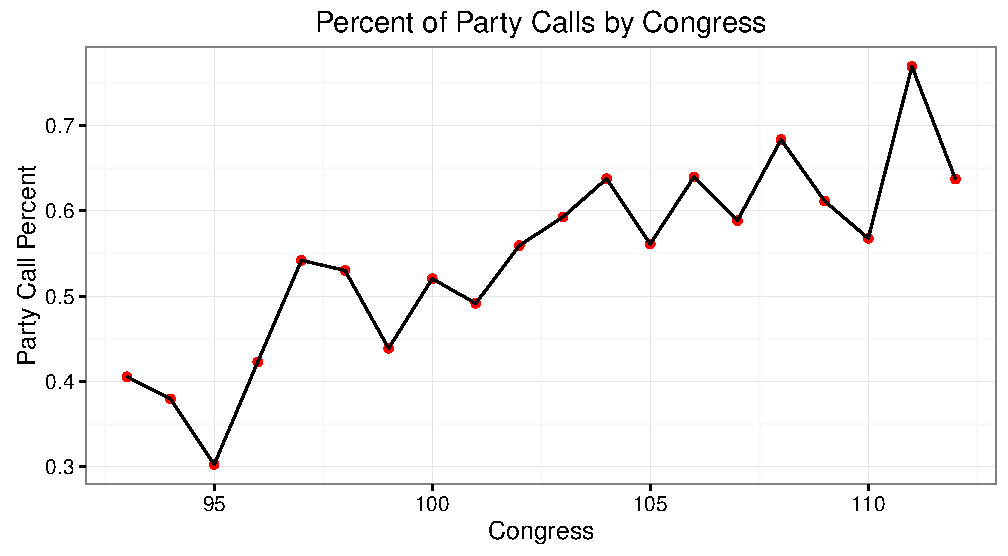
\includegraphics[width = \textwidth]{C:/Users/Ethan/Documents/GitHub/partycalls/plots/party_call_percent_plot_senate_lm.pdf}
\end{figure}

\begin{figure}[H]
	\centering
	\caption{Senate Ideological Extremism Coefficient Plot, Majority}
	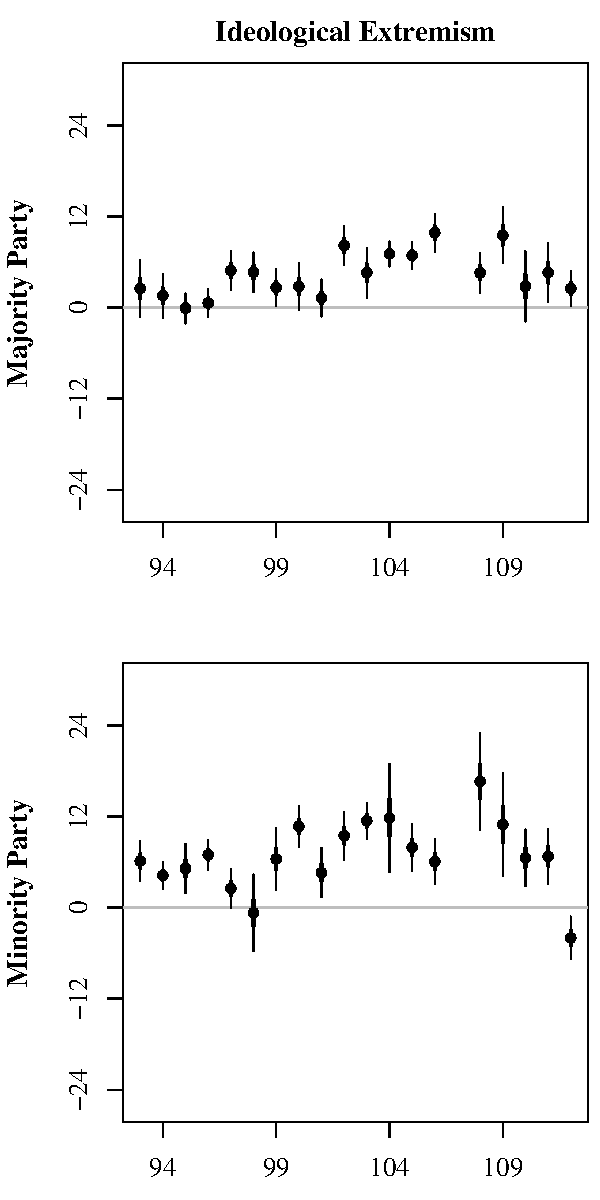
\includegraphics[width = 10cm]{C:/Users/Ethan/Documents/GitHub/partycalls/plots/senate-figure2-lm.pdf}
\end{figure}

\begin{figure}[H]
	\centering
	\caption{Senate Ideological Extremism Coefficient Plot, Party}
	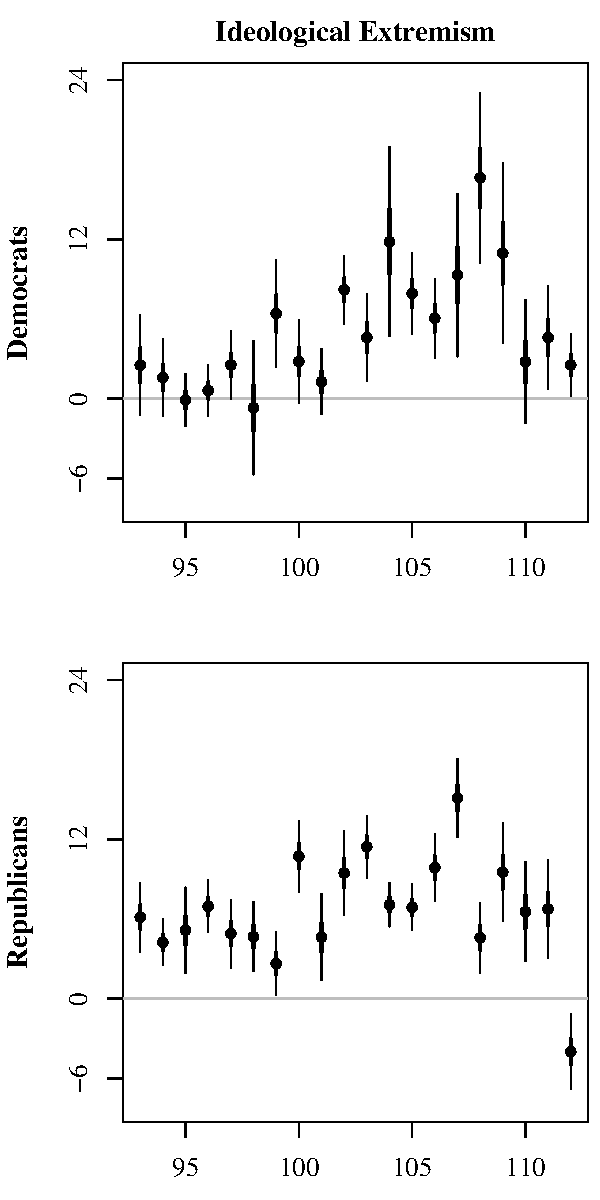
\includegraphics[width = 10cm]{C:/Users/Ethan/Documents/GitHub/partycalls/plots/senate-figure2-party.pdf}
\end{figure}

\begin{figure}[H]
	\centering
	\caption{Senate Ideological Extremism Coefficient Plot, Election Proximity}
	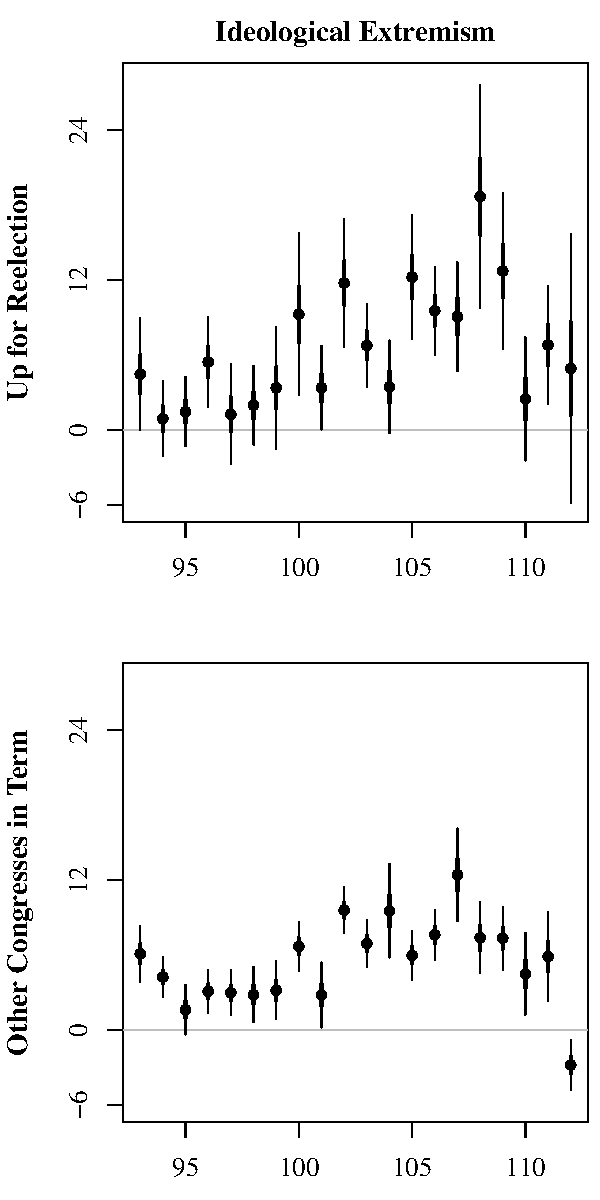
\includegraphics[width = 10cm]{C:/Users/Ethan/Documents/GitHub/partycalls/plots/senate-figure2-reelection.pdf}
\end{figure}

\begin{table}
	\begin{center}
		\caption{Senate Aggregate Regression Models}
		\begin{tabular}{l c c c c }
			\hline
			& Democrats & Republicans & Majority & Minority \\
			\hline
			ideological\_extremism & $3.136^{***}$  & $7.792^{***}$   & $4.708^{***}$  & $7.949^{***}$ \\
			& $(0.409)$      & $(0.357)$       & $(0.315)$      & $(0.400)$     \\
			chair                  & $0.852$        & $3.626^{***}$   & $-0.017$       &               \\
			& $(0.543)$      & $(0.700)$       & $(0.517)$      &               \\
			pfrate100              & $0.759^{***}$  & $0.742^{***}$   & $0.702^{***}$  & $0.702^{***}$ \\
			& $(0.030)$      & $(0.031)$       & $(0.025)$      & $(0.035)$     \\
			pres\_vote\_share      & $23.381^{***}$ & $-13.374^{***}$ & $18.213^{***}$ & $0.566$       \\
			& $(2.399)$      & $(3.082)$       & $(1.970)$      & $(3.187)$     \\
			south                  & $-1.690^{**}$  & $0.872$         & $0.054$        & $1.085$       \\
			& $(0.557)$      & $(0.578)$       & $(0.427)$      & $(0.622)$     \\
			power\_committee       & $-0.855$       & $-0.325$        & $-0.052$       & $-1.468$      \\
			& $(0.772)$      & $(0.924)$       & $(0.719)$      & $(1.064)$     \\
			vote\_share            & $-5.257^{*}$   & $14.914^{***}$  & $-1.178$       & $7.599^{*}$   \\
			& $(2.161)$      & $(2.802)$       & $(2.066)$      & $(2.958)$     \\
			female                 & $1.690^{*}$    & $0.451$         & $0.532$        & $4.256^{***}$ \\
			& $(0.730)$      & $(1.132)$       & $(0.758)$      & $(1.113)$     \\
			afam                   & $-1.164$       & $-10.789^{*}$   & $1.531$        & $-5.519$      \\
			& $(2.789)$      & $(4.278)$       & $(4.184)$      & $(3.219)$     \\
			latino                 & $1.814$        & $7.264^{**}$    & $4.781^{*}$    & $6.253$       \\
			& $(2.198)$      & $(2.779)$       & $(1.878)$      & $(3.506)$     \\
			up\_for\_reelection    & $-0.630$       & $-1.436^{**}$   & $-0.951^{*}$   & $-1.204^{*}$  \\
			& $(0.426)$      & $(0.538)$       & $(0.411)$      & $(0.603)$     \\
			seniority              & $0.041$        & $-0.024$        & $0.077$        & $0.118$       \\
			& $(0.052)$      & $(0.072)$       & $(0.060)$      & $(0.070)$     \\
			freshman               & $0.769$        & $0.358$         & $0.600$        & $0.996$       \\
			& $(0.708)$      & $(0.842)$       & $(0.631)$      & $(1.032)$     \\
			retiree                & $1.599$        & $2.290^{*}$     & $1.816^{*}$    & $2.575^{*}$   \\
			& $(0.897)$      & $(0.997)$       & $(0.850)$      & $(1.110)$     \\
			best\_committee        & $0.237$        & $0.008$         & $0.027$        & $0.373^{*}$   \\
			& $(0.124)$      & $(0.154)$       & $(0.118)$      & $(0.174)$     \\
			leader                 & $2.218^{**}$   & $0.910$         & $1.441^{*}$    & $1.940^{*}$   \\
			& $(0.712)$      & $(0.776)$       & $(0.661)$      & $(0.899)$     \\
			(Intercept)            & $9.447^{**}$   & $18.182^{***}$  & $16.365^{***}$ & $10.799^{**}$ \\
			& $(2.906)$      & $(3.489)$       & $(2.644)$      & $(4.009)$     \\
			\hline
			R$^2$                  & 0.689          & 0.641           & 0.684          & 0.615         \\
			Adj. R$^2$             & 0.684          & 0.635           & 0.679          & 0.608         \\
			Num. obs.              & 1042           & 951             & 1052           & 843           \\
			RMSE                   & 6.118          & 7.255           & 5.865          & 7.749         \\
			\hline
			\multicolumn{5}{l}{\scriptsize{$^{***}p<0.001$, $^{**}p<0.01$, $^*p<0.05$}}
		\end{tabular}
	\end{center}
\end{table}

\begin{table}
	\begin{center}
		\caption{Senate Intra Party Division Models}
		\begin{tabular}{l c c c c }
			\hline
			& \multicolumn{2}{c}{Democrats} & \multicolumn{2}{c}{Republicans} \\
			\cline{2-5}
			& Southern  & Others & Gingrich Senators & Others \\
			\hline
			ideological\_extremism & $4.519^{***}$  & $2.629^{***}$  & $3.012^{***}$  & $6.526^{***}$ \\
			& $(1.154)$      & $(0.409)$      & $(0.645)$      & $(0.401)$     \\
			south                  &                &                & $0.020$        & $1.011$       \\
			&                &                & $(0.707)$      & $(0.661)$     \\
			pfrate100              & $0.850^{***}$  & $0.634^{***}$  & $0.244^{***}$  & $0.827^{***}$ \\
			& $(0.065)$      & $(0.035)$      & $(0.050)$      & $(0.034)$     \\
			pres\_vote\_share      & $26.709^{***}$ & $22.988^{***}$ & $0.574$        & $-5.288$      \\
			& $(5.097)$      & $(2.641)$      & $(4.618)$      & $(3.425)$     \\
			vote\_share            & $-2.777$       & $-3.334$       & $2.376$        & $9.541^{**}$  \\
			& $(3.714)$      & $(2.827)$      & $(3.508)$      & $(3.208)$     \\
			latino                 &                & $2.774$        & $2.907$        & $3.419$       \\
			&                & $(1.968)$      & $(2.520)$      & $(3.613)$     \\
			female                 & $0.215$        & $2.476^{***}$  &                & $1.921$       \\
			& $(1.988)$      & $(0.735)$      &                & $(1.120)$     \\
			up\_for\_reelection    & $-1.548$       & $-0.343$       & $-0.466$       & $-1.785^{**}$ \\
			& $(1.073)$      & $(0.432)$      & $(0.698)$      & $(0.585)$     \\
			seniority              & $-0.295^{*}$   & $0.136^{*}$    & $-0.264$       & $0.139$       \\
			& $(0.140)$      & $(0.054)$      & $(0.178)$      & $(0.075)$     \\
			freshman               & $2.037$        & $0.699$        & $-0.198$       & $0.141$       \\
			& $(1.768)$      & $(0.725)$      & $(0.967)$      & $(0.968)$     \\
			retiree                & $1.653$        & $1.935^{*}$    & $2.811$        & $2.406^{*}$   \\
			& $(2.255)$      & $(0.924)$      & $(1.609)$      & $(1.049)$     \\
			best\_committee        & $0.575$        & $0.132$        & $0.081$        & $0.044$       \\
			& $(0.307)$      & $(0.129)$      & $(0.182)$      & $(0.177)$     \\
			leader                 & $5.755^{*}$    & $1.792^{**}$   & $1.892$        & $0.965$       \\
			& $(2.307)$      & $(0.694)$      & $(1.127)$      & $(0.836)$     \\
			power\_committee       & $0.722$        & $-1.360$       & $1.075$        & $-1.242$      \\
			& $(2.107)$      & $(0.779)$      & $(1.119)$      & $(1.058)$     \\
			chair                  & $3.093^{*}$    & $0.581$        & $1.291$        & $3.690^{***}$ \\
			& $(1.400)$      & $(0.555)$      & $(1.113)$      & $(0.739)$     \\
			afam                   &                & $-1.012$       &                & $-7.873$      \\
			&                & $(2.493)$      &                & $(4.193)$     \\
			(Intercept)            & $-6.288$       & $20.478^{***}$ & $67.769^{***}$ & $8.912^{*}$   \\
			& $(6.586)$      & $(3.184)$      & $(5.039)$      & $(3.890)$     \\
			\hline
			R$^2$                  & 0.728          & 0.571          & 0.236          & 0.678         \\
			Adj. R$^2$             & 0.713          & 0.563          & 0.174          & 0.671         \\
			Num. obs.              & 246            & 796            & 188            & 763           \\
			RMSE                   & 7.334          & 5.445          & 4.067          & 7.090         \\
			\hline
			\multicolumn{5}{l}{\scriptsize{$^{***}p<0.001$, $^{**}p<0.01$, $^*p<0.05$}}
		\end{tabular}
	\end{center}
\end{table}

\subsection{House}

% Table created by stargazer v.5.2 by Marek Hlavac, Harvard University. E-mail: hlavac at fas.harvard.edu
% Date and time: Mon, Mar 06, 2017 - 12:41:20
\begin{table}[H] \centering 
	\caption{} 
	\label{} 
	\begin{tabular}{@{\extracolsep{5pt}}lccccc} 
		\\[-1.8ex]\hline 
		\hline \\[-1.8ex] 
		Statistic & \multicolumn{1}{c}{N} & \multicolumn{1}{c}{Mean} & \multicolumn{1}{c}{St. Dev.} & \multicolumn{1}{c}{Min} & \multicolumn{1}{c}{Max} \\ 
		\hline \\[-1.8ex] 
		congress & 8,544 & 102.546 & 5.787 & 93 & 112 \\ 
		icpsrLegis & 8,544 & 18,470.740 & 9,043.958 & 62 & 99,342 \\ 
		state\_cd & 8,544 & 2,455.331 & 1,433.201 & 101 & 5,001 \\ 
		cd & 8,544 & 9.837 & 9.760 & 1 & 53 \\ 
		dem & 8,544 & 0.555 & 0.497 & 0 & 1 \\ 
		majority & 8,544 & 0.574 & 0.495 & 0 & 1 \\ 
		female & 8,544 & 0.094 & 0.292 & 0 & 1 \\ 
		afam & 8,544 & 0.063 & 0.244 & 0 & 1 \\ 
		latino & 8,544 & 0.035 & 0.183 & 0 & 1 \\ 
		votepct & 8,544 & 68.266 & 13.793 & 36 & 100 \\ 
		speaker & 8,544 & 0.002 & 0.042 & 0 & 1 \\ 
		chair & 8,544 & 0.051 & 0.219 & 0 & 1 \\ 
		subchr & 8,544 & 0.250 & 0.433 & 0 & 1 \\ 
		power & 8,544 & 0.255 & 0.436 & 0 & 1 \\ 
		seniority & 8,544 & 5.331 & 4.054 & 1 & 29 \\ 
		maj\_leader & 8,544 & 0.017 & 0.130 & 0 & 1 \\ 
		min\_leader & 8,544 & 0.019 & 0.137 & 0 & 1 \\ 
		south & 8,544 & 0.296 & 0.456 & 0 & 1 \\ 
		les & 8,544 & 1.008 & 1.595 & 0.000 & 18.686 \\ 
		drop & 8,544 & 0.000 & 0.000 & 0 & 0 \\ 
		freshman & 8,544 & 0.156 & 0.363 & 0 & 1 \\ 
		leader & 8,544 & 0.036 & 0.187 & 0 & 1 \\ 
		fips & 8,544 & 28.080 & 15.537 & 1 & 56 \\ 
		state\_alphabetical\_order & 8,544 & 24.455 & 14.349 & 1 & 50 \\ 
		dpres & 8,544 & 48.834 & 13.950 & 13.170 & 96.060 \\ 
		pres\_votepct & 8,544 & 56.562 & 12.365 & 16.310 & 96.060 \\ 
		bestgrosswart & 8,544 & 13.822 & 6.376 & 0 & 22 \\ 
		party\_free\_ideal\_point & 8,544 & $-$0.004 & 1.003 & $-$4.076 & 9.347 \\ 
		pirate100 & 8,544 & 85.800 & 11.478 & 8.021 & 100.000 \\ 
		pfrate100 & 8,544 & 86.955 & 7.507 & 0.000 & 100.000 \\ 
		ideological\_extremism & 8,544 & 0.603 & 0.802 & $-$4.317 & 9.347 \\ 
		\hline \\[-1.8ex] 
	\end{tabular} 
\end{table} 

% Table created by stargazer v.5.2 by Marek Hlavac, Harvard University. E-mail: hlavac at fas.harvard.edu
% Date and time: Mon, Mar 06, 2017 - 12:48:32
\begin{table}[!htbp] \centering 
	\caption{} 
	\label{} 
	\begin{tabular}{@{\extracolsep{5pt}}lccccc} 
		\\[-1.8ex]\hline 
		\hline \\[-1.8ex] 
		Statistic & \multicolumn{1}{c}{N} & \multicolumn{1}{c}{Mean} & \multicolumn{1}{c}{St. Dev.} & \multicolumn{1}{c}{Min} & \multicolumn{1}{c}{Max} \\ 
		\hline \\[-1.8ex] 
		congress & 4,746 & 102.059 & 5.785 & 93 & 112 \\ 
		icpsrLegis & 4,746 & 17,626.680 & 8,603.223 & 62 & 95,415 \\ 
		state\_cd & 4,746 & 2,476.726 & 1,422.596 & 102 & 5,001 \\ 
		cd & 4,746 & 9.596 & 9.070 & 1 & 53 \\ 
		dem & 4,746 & 1.000 & 0.000 & 1 & 1 \\ 
		majority & 4,746 & 0.700 & 0.458 & 0 & 1 \\ 
		female & 4,746 & 0.114 & 0.317 & 0 & 1 \\ 
		afam & 4,746 & 0.112 & 0.316 & 0 & 1 \\ 
		latino & 4,746 & 0.050 & 0.217 & 0 & 1 \\ 
		votepct & 4,746 & 70.230 & 14.571 & 36 & 100 \\ 
		speaker & 4,746 & 0.002 & 0.041 & 0 & 1 \\ 
		chair & 4,746 & 0.062 & 0.240 & 0 & 1 \\ 
		subchr & 4,746 & 0.321 & 0.467 & 0 & 1 \\ 
		power & 4,746 & 0.257 & 0.437 & 0 & 1 \\ 
		seniority & 4,746 & 5.752 & 4.376 & 1 & 29 \\ 
		maj\_leader & 4,746 & 0.019 & 0.136 & 0 & 1 \\ 
		min\_leader & 4,746 & 0.015 & 0.122 & 0 & 1 \\ 
		south & 4,746 & 0.289 & 0.453 & 0 & 1 \\ 
		les & 4,746 & 1.113 & 1.702 & 0.000 & 18.686 \\ 
		drop & 4,746 & 0.000 & 0.000 & 0 & 0 \\ 
		freshman & 4,746 & 0.140 & 0.347 & 0 & 1 \\ 
		leader & 4,746 & 0.034 & 0.182 & 0 & 1 \\ 
		fips & 4,746 & 28.318 & 15.433 & 1 & 56 \\ 
		state\_alphabetical\_order & 4,746 & 24.671 & 14.239 & 1 & 50 \\ 
		dpres & 4,746 & 54.871 & 14.495 & 16.310 & 96.060 \\ 
		pres\_votepct & 4,746 & 54.846 & 14.503 & 16.310 & 96.060 \\ 
		bestgrosswart & 4,746 & 13.832 & 6.398 & 0 & 22 \\ 
		party\_free\_ideal\_point & 4,746 & $-$0.546 & 0.809 & $-$4.076 & 4.317 \\ 
		pirate100 & 4,746 & 86.290 & 12.110 & 8.021 & 100.000 \\ 
		pfrate100 & 4,746 & 86.996 & 7.214 & 0.000 & 100.000 \\ 
		ideological\_extremism & 4,746 & 0.546 & 0.809 & $-$4.317 & 4.076 \\ 
		\hline \\[-1.8ex] 
	\end{tabular} 
\end{table} 

% Table created by stargazer v.5.2 by Marek Hlavac, Harvard University. E-mail: hlavac at fas.harvard.edu
% Date and time: Mon, Mar 06, 2017 - 12:48:34
\begin{table}[!htbp] \centering 
	\caption{} 
	\label{} 
	\begin{tabular}{@{\extracolsep{5pt}}lccccc} 
		\\[-1.8ex]\hline 
		\hline \\[-1.8ex] 
		Statistic & \multicolumn{1}{c}{N} & \multicolumn{1}{c}{Mean} & \multicolumn{1}{c}{St. Dev.} & \multicolumn{1}{c}{Min} & \multicolumn{1}{c}{Max} \\ 
		\hline \\[-1.8ex] 
		congress & 3,798 & 103.154 & 5.732 & 93 & 112 \\ 
		icpsrLegis & 3,798 & 19,525.480 & 9,462.085 & 226 & 99,342 \\ 
		state\_cd & 3,798 & 2,428.596 & 1,446.085 & 101 & 5,001 \\ 
		cd & 3,798 & 10.139 & 10.553 & 1 & 52 \\ 
		dem & 3,798 & 0.000 & 0.000 & 0 & 0 \\ 
		majority & 3,798 & 0.416 & 0.493 & 0 & 1 \\ 
		female & 3,798 & 0.069 & 0.254 & 0 & 1 \\ 
		afam & 3,798 & 0.002 & 0.049 & 0 & 1 \\ 
		latino & 3,798 & 0.016 & 0.126 & 0 & 1 \\ 
		votepct & 3,798 & 65.812 & 12.324 & 37 & 100 \\ 
		speaker & 3,798 & 0.002 & 0.043 & 0 & 1 \\ 
		chair & 3,798 & 0.037 & 0.189 & 0 & 1 \\ 
		subchr & 3,798 & 0.161 & 0.367 & 0 & 1 \\ 
		power & 3,798 & 0.251 & 0.434 & 0 & 1 \\ 
		seniority & 3,798 & 4.805 & 3.543 & 1 & 21 \\ 
		maj\_leader & 3,798 & 0.015 & 0.121 & 0 & 1 \\ 
		min\_leader & 3,798 & 0.024 & 0.153 & 0 & 1 \\ 
		south & 3,798 & 0.304 & 0.460 & 0 & 1 \\ 
		les & 3,798 & 0.876 & 1.439 & 0.000 & 17.547 \\ 
		drop & 3,798 & 0.000 & 0.000 & 0 & 0 \\ 
		freshman & 3,798 & 0.176 & 0.381 & 0 & 1 \\ 
		leader & 3,798 & 0.039 & 0.193 & 0 & 1 \\ 
		fips & 3,798 & 27.783 & 15.662 & 1 & 56 \\ 
		state\_alphabetical\_order & 3,798 & 24.185 & 14.482 & 1 & 50 \\ 
		dpres & 3,798 & 41.290 & 8.534 & 13.170 & 76.530 \\ 
		pres\_votepct & 3,798 & 58.707 & 8.537 & 23.470 & 86.830 \\ 
		bestgrosswart & 3,798 & 13.810 & 6.349 & 0 & 22 \\ 
		party\_free\_ideal\_point & 3,798 & 0.674 & 0.786 & $-$2.473 & 9.347 \\ 
		pirate100 & 3,798 & 85.186 & 10.605 & 31.276 & 100.000 \\ 
		pfrate100 & 3,798 & 86.904 & 7.858 & 28.302 & 100.000 \\ 
		ideological\_extremism & 3,798 & 0.674 & 0.786 & $-$2.473 & 9.347 \\ 
		\hline \\[-1.8ex] 
	\end{tabular} 
\end{table} 

% latex table generated in R 3.3.2 by xtable 1.8-2 package
% Thu Feb 23 17:39:42 2017
\begin{table}[H]
	\centering
	\caption{House Sorting Algorithm Coefficient Signs}
	\begin{tabular}{rrr}
		\hline
		& ($-$) Ideal & (+) Ideal \\ 
		\hline
		(-) Party & 0.38 & 0.15 \\ 
		(+) Party & 0.17 & 0.30 \\ 
		\hline
	\end{tabular}
\end{table}

\begin{figure}[H]
	\centering
	\caption{House Party Calls by Congress}
	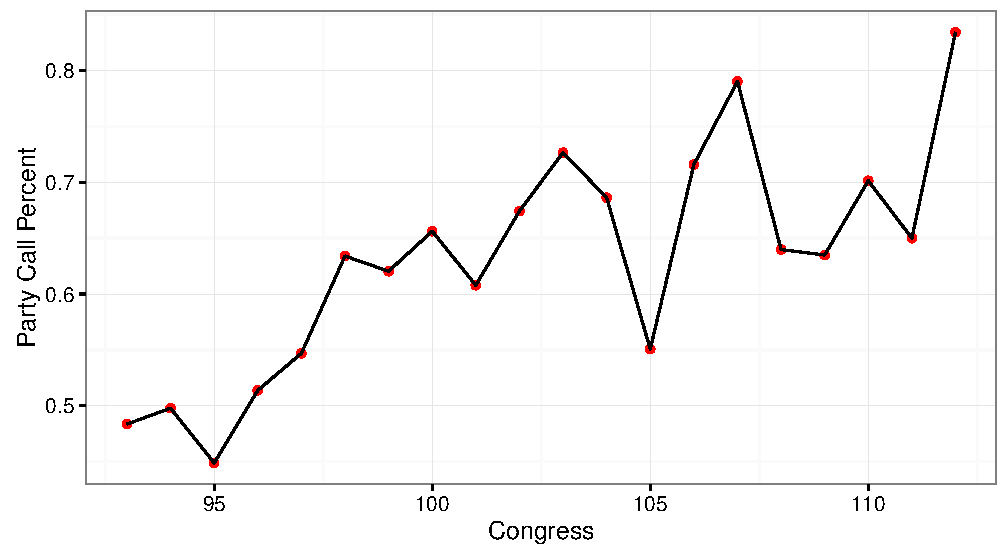
\includegraphics[width = \textwidth]{C:/Users/Ethan/Documents/GitHub/partycalls/plots/party_call_percent_plot_house_lm.pdf}
\end{figure}

\begin{figure}[H]
	\centering
	\caption{House Ideological Extremism Coefficient Plot, Majority}
	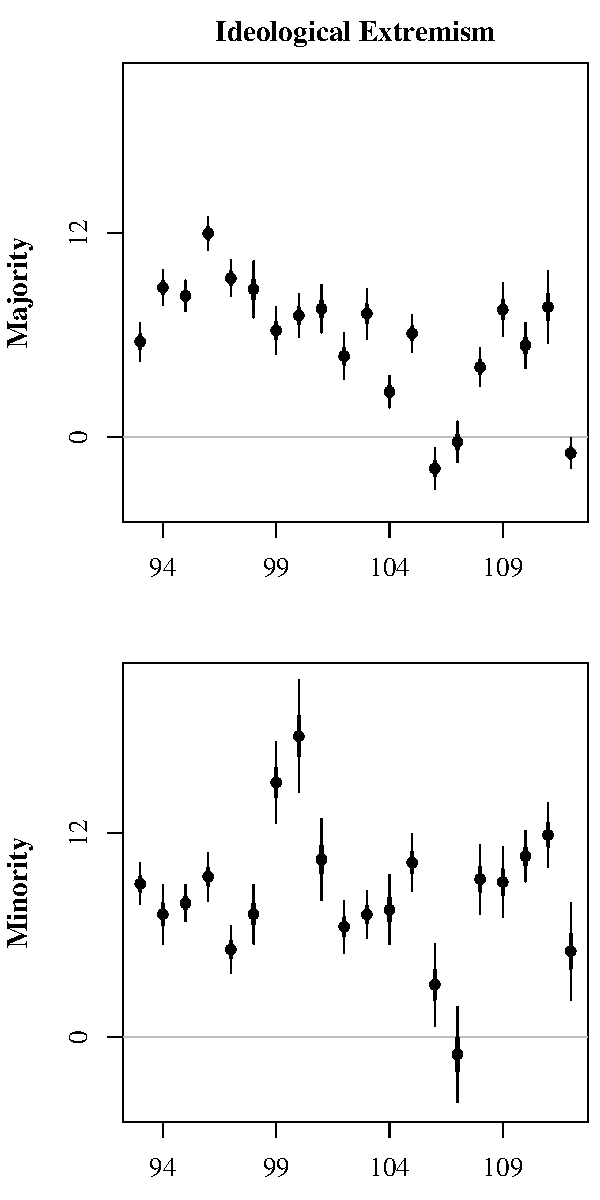
\includegraphics[width = 10cm]{C:/Users/Ethan/Documents/GitHub/partycalls/plots/who-heeds-figure2-replication_lm.pdf}
\end{figure}

\begin{figure}[H]
	\centering
	\caption{House Ideological Extremism Coefficient Plot, Party}
	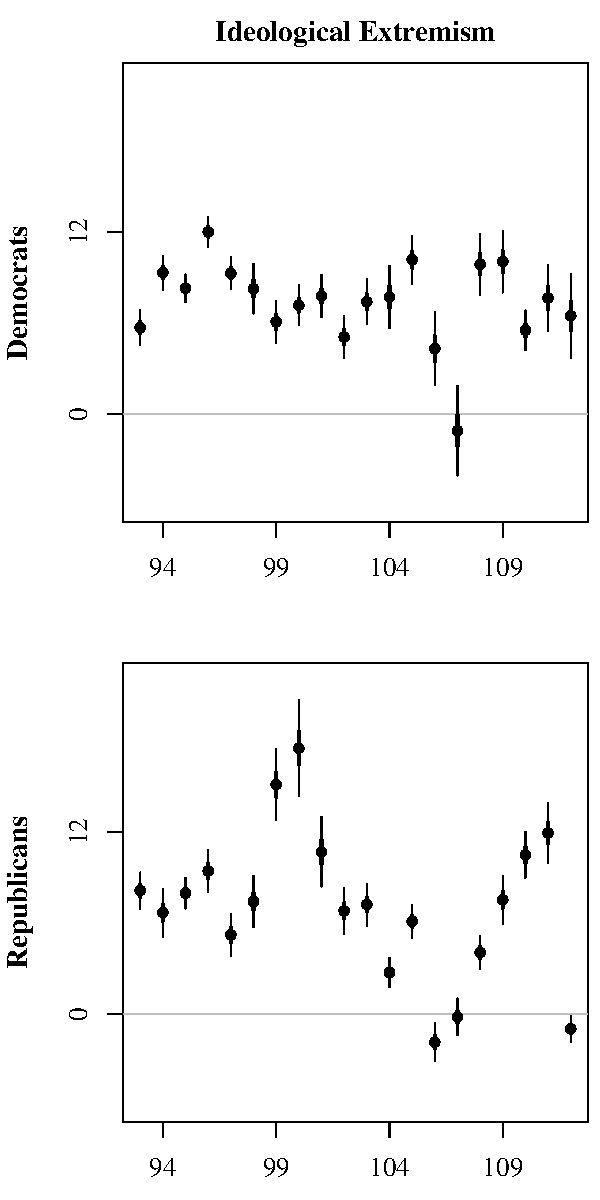
\includegraphics[width = 10cm]{C:/Users/Ethan/Documents/GitHub/partycalls/plots/who-heeds-figure2-replication_party.pdf}
\end{figure}

\begin{table}
	\begin{center}
		\caption{House Aggregate Regression Models}
		\begin{tabular}{l c c c c }
			\hline
			& Democrats & Republicans & Majority & Minority \\
			\hline
			ideological\_extremism & $8.34^{***}$  & $5.84^{***}$  & $6.64^{***}$  & $8.73^{***}$  \\
			& $(0.17)$      & $(0.21)$      & $(0.16)$      & $(0.20)$      \\
			pfrate100              & $0.64^{***}$  & $0.41^{***}$  & $0.52^{***}$  & $0.63^{***}$  \\
			& $(0.02)$      & $(0.02)$      & $(0.01)$      & $(0.02)$      \\
			pres\_votepct          & $0.09^{***}$  & $-0.09^{***}$ & $0.20^{***}$  & $0.16^{***}$  \\
			& $(0.01)$      & $(0.02)$      & $(0.01)$      & $(0.02)$      \\
			south                  & $-2.43^{***}$ & $3.63^{***}$  & $-1.65^{***}$ & $-0.36$       \\
			& $(0.28)$      & $(0.34)$      & $(0.25)$      & $(0.31)$      \\
			votepct                & $-0.04^{***}$ & $-0.00$       & $-0.09^{***}$ & $-0.06^{***}$ \\
			& $(0.01)$      & $(0.01)$      & $(0.01)$      & $(0.01)$      \\
			female                 & $0.53$        & $-0.08$       & $-0.13$       & $2.13^{***}$  \\
			& $(0.35)$      & $(0.57)$      & $(0.40)$      & $(0.44)$      \\
			afam                   & $-0.52$       & $5.01$        & $-3.04^{***}$ & $3.24^{***}$  \\
			& $(0.44)$      & $(2.97)$      & $(0.53)$      & $(0.61)$      \\
			latino                 & $1.73^{***}$  & $2.41^{*}$    & $2.83^{***}$  & $3.02^{***}$  \\
			& $(0.51)$      & $(1.15)$      & $(0.63)$      & $(0.70)$      \\
			seniority              & $0.05$        & $-0.33^{***}$ & $0.02$        & $0.00$        \\
			& $(0.03)$      & $(0.05)$      & $(0.03)$      & $(0.04)$      \\
			freshman               & $-0.07$       & $1.00^{*}$    & $0.28$        & $-0.39$       \\
			& $(0.36)$      & $(0.46)$      & $(0.35)$      & $(0.44)$      \\
			bestgrosswart          & $-0.04^{*}$   & $-0.24^{***}$ & $-0.17^{***}$ & $-0.16^{***}$ \\
			& $(0.02)$      & $(0.03)$      & $(0.02)$      & $(0.02)$      \\
			leader                 & $1.96^{**}$   & $2.80^{***}$  & $2.62^{***}$  & $1.79^{**}$   \\
			& $(0.60)$      & $(0.76)$      & $(0.65)$      & $(0.65)$      \\
			power                  & $1.82^{***}$  & $2.95^{***}$  & $3.02^{***}$  & $1.06^{**}$   \\
			& $(0.28)$      & $(0.37)$      & $(0.27)$      & $(0.36)$      \\
			chair                  & $2.49^{***}$  & $9.85^{***}$  & $1.85^{***}$  &               \\
			& $(0.50)$      & $(0.80)$      & $(0.44)$      &               \\
			(Intercept)            & $24.00^{***}$ & $53.04^{***}$ & $36.42^{***}$ & $17.78^{***}$ \\
			& $(1.58)$      & $(2.21)$      & $(1.49)$      & $(2.05)$      \\
			\hline
			R$^2$                  & 0.63          & 0.30          & 0.57          & 0.48          \\
			Adj. R$^2$             & 0.63          & 0.30          & 0.56          & 0.48          \\
			Num. obs.              & 4746          & 3798          & 4902          & 3642          \\
			RMSE                   & 7.36          & 8.87          & 7.55          & 8.01          \\
			\hline
			\multicolumn{5}{l}{\scriptsize{$^{***}p<0.001$, $^{**}p<0.01$, $^*p<0.05$}}
		\end{tabular}
	\end{center}
\end{table}

\begin{table}
	\begin{center}
		\caption{Minozzi Volden (2013) Table 3 Replication}
		\begin{tabular}{l c c c c c c }
			\hline
			& \multicolumn{3}{c}{Democrats} & \multicolumn{3}{c}{Republicans} \\
			\cline{2-7}
			Congress: &  97 & 102 & 107 & 97 & 102 & 107 \\
			\hline
			ideological\_extremism & $9.27^{***}$  & $5.07^{***}$  & $-1.11$      & $5.21^{***}$ & $6.78^{***}$  & $-0.20$       \\
			& $(0.53)$      & $(0.69)$      & $(1.50)$     & $(0.71)$     & $(0.76)$      & $(0.61)$      \\
			pfrate100              & $1.03^{***}$  & $0.67^{***}$  & $1.11^{**}$  & $0.50^{***}$ & $0.48^{***}$  & $0.35^{**}$   \\
			& $(0.07)$      & $(0.08)$      & $(0.36)$     & $(0.08)$     & $(0.08)$      & $(0.11)$      \\
			pres\_votepct          & $0.15^{**}$   & $0.14^{**}$   & $0.22^{***}$ & $0.23^{***}$ & $0.21^{*}$    & $0.18^{***}$  \\
			& $(0.05)$      & $(0.05)$      & $(0.06)$     & $(0.07)$     & $(0.08)$      & $(0.03)$      \\
			south                  & $-4.20^{***}$ & $-1.31$       & $-3.13^{*}$  & $1.53$       & $0.07$        & $1.75^{***}$  \\
			& $(1.02)$      & $(0.80)$      & $(1.28)$     & $(1.19)$     & $(1.22)$      & $(0.52)$      \\
			votepct                & $-0.08^{*}$   & $-0.03$       & $-0.04$      & $0.05$       & $-0.00$       & $-0.03$       \\
			& $(0.03)$      & $(0.03)$      & $(0.05)$     & $(0.05)$     & $(0.03)$      & $(0.02)$      \\
			female                 & $0.05$        & $-1.58$       & $2.44^{*}$   & $-4.21^{*}$  & $-1.87$       & $-1.39$       \\
			& $(2.06)$      & $(1.22)$      & $(1.21)$     & $(2.00)$     & $(2.25)$      & $(0.83)$      \\
			afam                   & $-2.56$       & $-1.98$       & $-1.43$      &              & $3.95$        & $-3.54$       \\
			& $(2.12)$      & $(1.58)$      & $(1.73)$     &              & $(6.14)$      & $(3.57)$      \\
			latino                 & $4.02$        & $2.79$        & $0.69$       & $-1.28$      & $3.26$        & $0.79$        \\
			& $(2.91)$      & $(1.90)$      & $(1.89)$     & $(5.75)$     & $(6.35)$      & $(1.50)$      \\
			seniority              & $0.08$        & $0.07$        & $-0.11$      & $-0.02$      & $-0.71^{***}$ & $-0.17^{*}$   \\
			& $(0.12)$      & $(0.10)$      & $(0.13)$     & $(0.17)$     & $(0.15)$      & $(0.08)$      \\
			freshman               & $-1.25$       & $0.01$        & $-0.13$      & $3.45^{*}$   & $3.76^{*}$    & $0.59$        \\
			& $(1.43)$      & $(1.19)$      & $(2.02)$     & $(1.34)$     & $(1.77)$      & $(0.78)$      \\
			bestgrosswart          & $0.09$        & $-0.06$       & $0.25^{*}$   & $0.11$       & $0.11$        & $0.17^{**}$   \\
			& $(0.08)$      & $(0.08)$      & $(0.10)$     & $(0.09)$     & $(0.11)$      & $(0.05)$      \\
			leader                 & $7.02^{*}$    & $2.00$        & $0.56$       & $0.38$       & $4.26$        & $3.17^{*}$    \\
			& $(2.87)$      & $(1.95)$      & $(2.42)$     & $(2.42)$     & $(2.24)$      & $(1.23)$      \\
			power                  & $1.09$        & $1.44$        & $-1.23$      & $-1.37$      & $-0.03$       & $-0.21$       \\
			& $(1.02)$      & $(0.90)$      & $(1.31)$     & $(1.35)$     & $(1.41)$      & $(0.63)$      \\
			chair                  & $2.61$        & $1.31$        &              &              &               & $1.30$        \\
			& $(1.52)$      & $(1.35)$      &              &              &               & $(0.91)$      \\
			(Intercept)            & $-18.03^{**}$ & $25.29^{***}$ & $-33.70$     & $11.17$      & $23.11^{**}$  & $47.81^{***}$ \\
			& $(6.71)$      & $(7.32)$      & $(35.43)$    & $(8.06)$     & $(8.49)$      & $(10.27)$     \\
			\hline
			R$^2$                  & 0.82          & 0.65          & 0.36         & 0.54         & 0.61          & 0.52          \\
			Adj. R$^2$             & 0.80          & 0.64          & 0.31         & 0.50         & 0.58          & 0.49          \\
			Num. obs.              & 233           & 263           & 209          & 187          & 162           & 217           \\
			RMSE                   & 5.47          & 4.97          & 6.39         & 5.62         & 5.86          & 3.26          \\
			\hline
			\multicolumn{7}{l}{\scriptsize{$^{***}p<0.001$, $^{**}p<0.01$, $^*p<0.05$}}
		\end{tabular}
	\end{center}
\end{table}













\end{document}